\documentclass[12pt]{article}

\usepackage[authoryear]{natbib}
\usepackage{hyperref}
%\topmargin -1cm
%\oddsidemargin 0.3cm
%\evensidemargin 0cm
\usepackage[margin=1in]{geometry}
%\textwidth 16cm
%\textheight 22cm
\usepackage{epigraph}
\usepackage{amsmath}
\usepackage{amsfonts}
\usepackage{subfigure}
\usepackage{setspace}
\usepackage[multiple]{footmisc}
\usepackage{bm}
\usepackage{lscape}
\usepackage{graphicx}
\usepackage{amssymb}
\usepackage{amsthm}
\usepackage{lineno}
\usepackage{color}
\usepackage{xcolor}
\usepackage{csquotes}
\usepackage{enumitem}
\newtheorem{proposition}{Proposition}[section]
\newtheorem{lemma}{Lemma}[section]
\newtheorem{definition}{Definition}
\newtheorem{corollary}{Corollary}[section]
\newtheorem{result}{Result}
\numberwithin{equation}{section}
\usepackage{caption}
\usepackage{subcaption}
\usepackage{booktabs,threeparttable}
\newcommand\fnote[1]{\captionsetup{font=footnotesize}\caption*{#1}}
\usepackage{tikz}
\usetikzlibrary{patterns}
\setlist[enumerate]{itemsep=0pt}

%%% color setting
\definecolor{darkred}{rgb}{0.6, 0, 0}
\definecolor{ChadDarkBlue}{rgb}{.1,0,.2}  
\definecolor{ChadBlue}{rgb}{.1,.1,.65}  
\definecolor{ChadRoyal}{rgb}{.2,.2,.8}  
\definecolor{ChadGreen}{rgb}{0,.4,0}    % Dark Green
\definecolor{ChadRed}{rgb}{.6,.2,.2}
\hypersetup{
    colorlinks=true,  % Enable colored links
    linkcolor=ChadBlue,   % Color of internal links (like sections)
    citecolor=ChadBlue,   % Color of citation links
    filecolor=ChadBlue,   % Color of file links
    urlcolor=ChadBlue,    % Color of external links
    %refcolor=Chadred     % Color of reference links (if different from citecolor)
}

\usepackage{accents}
\newcommand{\ubar}[1]{\underaccent{\bar}{#1}}

\newgeometry{margin=1in}
\title{When Transparency Backfires:\\ Strategic Obfuscation and Financial Fragility\thanks{For helpful comments and discussions, we thank Zhi Da, Paul Ehling, Albert Kyle, Yasuto Monden, Don Noh, Yoshihiro Ohashi, Maureen O'Hara, Wataru Ohta, Norman Sch\"{urhoff}, Yung Chiang Yang, and seminar participants at Tokyo Metropolitan University and HKUST. All errors and omissions are our own.}}



\author{
  \makebox[\textwidth][c]{%
    \begin{minipage}{0.4\textwidth}
      \centering
      Jun Aoyagi\thanks{Department of Finance, Hong Kong University of Science and Technology, Clearwater Bay, Kowloon, Hong Kong. E-mail: junaoyagi@ust.hk.} \\ % Author AAA with their affiliation
      \small{HKUST} % Institution of AAA
    \end{minipage}
    \hspace{0.05\textwidth} % Space between the two authors
    \begin{minipage}{0.4\textwidth}
      \centering
      Yuki Sato\thanks{Department of Economics, Keio University, 2-15-45 Mita, Minato-ku, 109-8345 Tokyo, Japan. E-mail: yuki.sato@keio.jp.} \\ % Author BBB with their affiliation
      \small{Keio University} % Institution of BBB
    \end{minipage}
  }
  % \\[5pt]
  % \\ 
  % \makebox[\textwidth][c]{%
  %   \begin{minipage}{0.4\textwidth}
  %     \centering
  %     Raluca Toma\thanks{Peritus Investment Consultancy, Walchestrasse 23, CH-8006, Zürich, Switzerland. E-mail: raluca.toma@peritus.ch.} \\ % Author CCC with their affiliation
  %     \small{Peritus Investment Consultancy}\\[5pt] % Institution of CCC
  %   \end{minipage}
  % \vspace*{1.5cm}}
}


%\date
\begin{document}
\maketitle
\begin{abstract}
\normalsize
We study a model of delegated asset management in which a fund manager cares not only about trading profits but also about her reputation, captured by investors’ perceptions of the manager’s skill. The fund is intentionally made opaque by the manager, who communicates noisy information about her trading strategy to clients. This opacity generates two self-fulfilling equilibria: a benchmark equilibrium and a “flow-driven” equilibrium. In the benchmark equilibrium, the manager prioritizes fund performance, and her trading intensity is set at the profit-maximizing level. In contrast, in the flow-driven equilibrium, the manager trades more aggressively in order to appear skilled, thereby building reputation among investors and attracting larger fund flows, while the fund exhibits poor performance. Our results imply that (1) fund opacity and reputation concerns can trigger market fragility and increase inequality in managers’ compensation; (2) fund managers with different skill levels adopt different trading styles; and (3) skill in active management does not necessarily translate into superior performance. Our model also shows that highly skilled fund managers are more likely to choose opaque fund structures, as opacity makes it difficult to communicate trading strategies to investors and weakens incentives for reputation-driven risk-taking. In this sense, fund opacity serves as a commitment device that allows skilled managers to pursue profit-driven trading strategies rather than engaging in flashy risk-taking aimed at signaling high skill.

%We study a model of delegated asset management in which a fund manager care not only about trading profits but also her reputation, i.e., investors' perception of the manager's skill. Fund opacity, defined as imperfect information about the fund's strategy communicated to investors, generates two self-fulfilling equilibria: a benchmark and a “flow-driven” equilibrium. In the benchmark equilibrium, the manager prioritize the fund performance, and her trading intensity is at the profit-maximizing level. In the latter, however, the fund manager trades more aggressively to appear skilled, thereby establishing reputation among investors and attracting larger fund flow. The flow-driven equilibrium features an illiquid financial market, poorer fund performance, and higher price volatility. Our results suggest that (1) fund opacity and reputation concerns triggers market fragility and increasing inequality in managers' compensation; (2) fund managers with different skill levels adopt different trading styles; and (3) skills in active management may not translate into performance. We futher endogenize fund opacity and show that highly skilled fund managers tend to make their funds opaque, as opacity makes it difficult to communicate their trading strategy to investors, thereby serving as a commitment device to take a profit-driven trading strategy rather than engaging in flasy risk taking to show off their high skills. 

\end{abstract}
\vspace{10pt}
{\it JEL classification:} G11, G12, G14, G23\\[5pt]
{\it Key words:} informed trading, delegated asset management, opacity, reputation, financial fragility
\newpage
\newgeometry{margin=1.5in}


% in-paper disclosure statement
%\begin{center}\textbf{Conflict-of-interest disclosure statement}
\end{center}

\paragraph{Jun Aoyagi:} I have nothing to disclose.
\paragraph{Yuki Sato:} This work was supported by KAKENHI (Grants-in-Aid for Scientific Research) of JSPS (Japan Society for the Promotion of Science), FY 2017-2019. The Grant Number is JP17H07084, and the total amount is JPY 2,100,000 (about USD 14,000).
\paragraph{Raluca Toma:} I have nothing to disclose.
%\newpage

%\doublespacing
\onehalfspacing
%*==*==*==*==*==*==*==*==*==*==*==*==*==*==*
\section{Introduction}\label{sec:introduction}
Obfuscation is common in investor-directed fund communications.
Even when pursuing simple strategies, fund managers describe them in markedly different and often unnecessarily complex ways. For example, as \citet*{dehaan2021obfuscation} document, two funds that both track the S\&P 500 describe essentially identical objectives with strikingly different clarity: Schwab states in a single sentence, “The fund's goal is to track the total return of the S\&P 500 Index,” while Deutsche describes it in 60 words, embedding the same objective in technical language.\footnote{Deutsche's S\&P 500 index fund is described as “The fund seeks to provide investment results that, before expenses, correspond to the total return of common stocks publicly traded in the United States, as represented by the Standard \& Poor's 500 Composite Stock Price Index (S\&P 500 Index). The fund invests for capital appreciation, not income; any dividend and interest income is incidental to the pursuit of its objective.”} Similar patterns arise in fund names: labels such as “Dynamic Opportunity Fund,” “Flexible Growth Strategy,” or “Opportunistic Equity Fund” convey little concrete meaning to unprofessional retail investors at first glance, yet in practice often correspond to relatively simple large-cap portfolios that closely resemble the S\&P 500. This pattern is puzzling, as standard signaling theory suggests that managers, seeking to convey skill and attract capital, should prefer greater transparency rather than opacity.
Why would managers make information harder for their own investors to interpret, and what are the incentives and market consequences when fund opacity becomes a manager's strategic choice?

To address these questions, we study an equilibrium model of financial market trading with delegated asset management. A fund manager, privately informed about her skill, raises capital from investors through obfuscated communications and trades a risky asset in the financial market \`a la \citet{kyle1985continuous}. We define skill as the manager-specific ability to uncover more information about asset payoffs than the market: the more skilled the manager, the larger the mispricing she can identify and the greater the trading profits she can potentially earn. To attract fund flows, the manager privately communicates information about her risky position (portfolio) to investors. Investors, in turn, use this fund information to infer the manager's skill and decide on capital allocation to the fund. Importantly, the manager strategically chooses the readability of this communication: by obfuscating information, she makes it more difficult for investors to back out her underlying skill.\footnote{Following \citet*{ellison2009search}, the term ``obfuscation" refers to general practices that reduce the readability of information and distort communications. Accordingly, ``transparency" and ``opacity" refer to the degre of interpretability and precision of information with which investors can assess the fund’s positions, rather than mere disclosure.}

The model yields two stable, self-fulfilling equilibria regarding the manager's trading strategy. One of the equilibria is similar to that of \citet{kyle1985continuous}, where the manager employs the profit-maximizing trading strategy. In the other, which we call the “flow-driven” equilibrium, the manager trades the risky asset more aggressively to appear skilled and to attract large fund flows. This strategy increases trading volume, price volatility, and market liquidity but undermines the fund expected performance by revealing too much private information to the market maker.
Intuitively, the manager can boost investors' perception of her skill by placing a large order, either buy or sell, because such an action makes her appear like a skilled manager who has identified an asset with significant mispricing.
%\footnote{In equilibrium, investors accurately anticipate the manager's strategy, so their learning is not manipulated; nevertheless, the manager may take excessive risk following investors' belief that the manager trades more aggressively than the profit-maximizing level, as doing otherwise makes investors (incorrectly) infer a less skilled manager and reduce fund flows.} 
Although the expected performance deteriorates, it triggers large fund flows, and the manager earns a large fee income. Key to our multiple equilibria is the manager's conflicting motives for revealing skill: on one hand, she wishes to hide her skill from the market maker to earn trading profits, but on the other hand, she wants to show it off to investors to establish high reputation and attract large fund flows. 

The relative strength of these competing motives is governed by the degree of fund opacity. When opacity is high, investors can extract little information from fund communications and do not rely on them to infer skill. Thus, flows are insensitive to the manager's trading strategy, the showing-off motive is suppressed, and only the Kyle-like equilibrium survives. When opacity is low, investors rely heavily on fund information, and only the flow-driven equilibrium exists. At intermediate levels of opacity, however, both equilibria coexist, and which one prevails is determined by investors' beliefs. If investors expect aggressive, flow-driven trading, they treat fund information as a reliable signal of skill, making flows highly responsive to reported positions. It strengthens the showing-off motive and induces the manager to trade aggressively, confirming the investors' beliefs. The symmetric argument sustains the Kyle-like equilibrium when investors expect profit-maximizing behavior. A mere shift in beliefs, unaccompanied by any change in fundamentals, can therefore trigger a transition from the Kyle-like to the flow-driven equilibrium, where price volatility is high and trading performance is poor. We interpret this susceptibility to non-fundamental belief shifts as \textit{fragility}.\footnote{As in \citet{greenwood2011stock}, we define a market as fragile if it is susceptible to non-fundamental demand shifts, such as those caused by changes in investor beliefs.} 

%The equilibrium multiplicity in trading styles has implications for the fund-management industry. For example, the flow-driven equilibrium explains ovservations by \citet{philippon2012wages} and \citet{celerier2019returns}, who document increasing returns to talent and their significant contribution to income inequality in the finance industry. In the flow-driven equilibrium, managers' fee income exhibits greater inequality among high- and low-skilled managers compared to those in the Kyle-like equilibrium, as they trade aggressively and reveal their skills more than they do in the Kyle-like equilibrium. This allows investors to better assess each manager's skill and, therefore, to allocate capital more accurately according to managers' skills. Moreover, multiple equilibria offer a novel explanation for the puzzling relationship (or the lack thereof) between skill and persistent performance. In our model, skill does not translate into persistent performance, as high-skilled managers in the flow-driven equilibrium may underperform low-skilled ones following the Kyle-like equilibrium, consistent with the evidence documented in the empirical literature (e.g., \citealp*{busse2010performance}; \citealp{berk2004mutual}).

Building on these results, we endogenize fund opacity and study which types of managers contribute to financial fragility. By obfuscating fund information, a manager weakens investors' responsiveness to reported positions and curbs her showing-off incentive at the portfolio-decision stage. Although, when deciding on her risky position, she takes investors' belief-updating rule as given and is tempted to over-trade to attract flows, she can \textit{ex-ante} influence that rule through obfuscation. Opacity thus serves as a commitment device: by tying her own hands, the manager mitigates inefficient risk-taking, raises the profit margin of her risky position, and improves the fund's expected performance, thereby benefiting both herself and investors.

The value of this commitment is greater for higher-skilled managers, as they benefit more from improved profit margins. Optimal opacity therefore increases with managers' skill. This result is consistent with the ``brain drain'' documented by \citet{kostovetsky2017brain}, whereby top mutual fund managers migrate to more opaque hedge funds and deliver superior performance. Crucially, the relationship between opacity and fragility is non-monotone. While high opacity yields a unique Kyle-like equilibrium and low opacity yields a unique flow-driven equilibrium, it is at intermediate levels of opacity where multiple equilibria, and thus fragility, arise. Because intermediate-skilled managers optimally choose intermediate opacity, they expose financial markets to belief-driven instability. Such behavior is consistent with momentum crashes and sudden reversals observed during financial crises \citep{brunnermeier2009deciphering}, as well as the abrupt strategy unwinding among quantitative funds documented by \citet{khandani2011what}. Importantly, fragility in our model is driven entirely by shifts in market beliefs and can arise without fundamental shocks, in line with the argument that large historical price swings are rarely accompanied by proportionally large changes in fundamentals \citep{gennotte1999market}. A direct policy implication follows: transparency mandates may push managers toward lower opacity and move high-skilled managers into the fragile intermediate region, thereby \textit{increasing} rather than decreasing systemic fragility. Transparency, in this sense, backfires.

%% Literature Review %%
Our paper contributes to the understanding of opacity, complexity, and obfuscation in financial markets. Empirically, \citet*{edelen2012disclosure}, \citet*{badoera2020icansee}, and \citet*{dehaan2021obfuscation} document that mutual funds strategically obfuscate disclosures of their strategies and fee sturcutures, and \citet{celerier2019returns} show that structured financial products are deliberately made complex. Building on such evidence, \citet{carlin2009strategic}, \citet{carlin2010obfuscation}, and \citet{sato2014opacity} develop theoretical models in which complexity enables financial institutions to extract fees or preserve informational advantages. In these models, however, opacity is typically treated as technologically given or engineered externally, while we analyze its implications when fund managers strategically obfuscate. Moreover, opacity in our framework improves both managers’ and investors’ \textit{ex-ante} utility. Unlike the prior literature, managers obfuscate not to exploit less-informed investors, but because opacity serves as a commitment device that mitigates managers' showing-off motive in financial markets.

Our paper is also related to the literature on fragility and trading frenzies in financial markets. \citet{cespa2015beauty} is most closely related, as they also find multiple equilibria arising from short-term investor horizons and persistent liquidity trading. In \citet*{froot1992herd}, strategic complementarities among short-term traders are also important for the emergence of multiple equilibria. Unlike these studies, our model does not feature short horizons; instead, we obtain fragility from managers conserns about fund flows. In \citet{cespa2014illiquidity}, learning from other assets amplifies shocks and causes liquidity crashes. Although the mechanism is different, our model can also result in liquidity crashes when the economy switches between equilibria due to non-fundamental shocks. Also, several studeits, such as \citet{veldkamp2006media} and \citet*{goldstein2013trading}, features trading frenzies based on strategic complementarities in information markets or a feedback effect from financial markets to a firm's real investment. By contrast, in our flow-driven equilibrium, a fund manager trades aggressively out of fear of being perceived as less skilled by the recruiter who believes that she would trade aggressively. 

Lastly, our work contributes to the broader understanding of the role of asymmetric information about skills in financial markets. \citet{Huberman1993ontheincentives}, \citet{huddart1999reputation}, \citet{di2015fake}, \citet*{malliaris2021reputation}, and \citet*{bijlsma2018competition} derive implications for the risk-taking behavior of agents when ability is private information but is conveyed to investors through signals, such as realized performance. In the context of the principal-agent proglem, \citet{prat2005wrong} shows that transparency in such communications can be detrimental, as it distorts agents' behavior. We also link trader skill to private information and asset markets; however, unlike these papers, our focus is on deriving pricing implications and managers' incentive to obfuscate fund information. \citet{guerrieri2012fund} show that career concerns amplify price volatility, similar to our findings. In \citet{dasgupta2006financial}, career concerns lead to churning (trading without private information), and in \citet{dasgupta2008information}, they lead to herding (ignoring private information and trading like everyone else). These three papers are closely related to ours in that they study career concerns and endogenous asset prices, but they do not analyze fragility and endogenous fund opacity, the main focus of our paper. \citet{gervais2020transparency} consider managers’ transparency choices under exogenous transparency costs and obtain sorting across skill types. By contrast, we derive an endogenous cost of transparency arising from flow-driven trading distortions. As a result, transparency in our model does not merely separate types but alters trading behavior and can generate belief-driven multiple equilibria and market fragility.

The rest of the paper proceeds as follows. Section \ref{sec:Model} presents a baseline model with exogenous reputation concerns, and Section \ref{sec:eqm} studies the equilibrium. Section \ref{sec:endogenous} endogenizes reputation concerns by introducing a two-period model and presents the implications of our results. Section \ref{sec:skillacquisition} analyzes traders' skill acquisition. The \hyperref[app:appendix]{Online Appendix} contains all proofs for the theoretical results.
\section{Model}\label{sec:Model}
%===========================================
This section presents a one-period trading model à la \citet{kyle1985continuous} with delegated asset management. 

\subsection{Setting}
The economy consists of a \textit{fund manager}, a competitive \textit{market maker}, a \textit{noise trader}, and $n\ge 2$ of \textit{investors}. All players are risk neutral. The manager leverages her skill (defined later) to identify a single risky asset with potential mispricing, raises capital from investors, and allocates it between the risky asset and a risk-free asset with a zero interest rate.\footnote{We abstract away from information acquisition by individual investors and assume that they invest through a manager due to the lack of informational advantages. This assumption would be supported by, for example, information- or skill-acquisition costs, where only the fund manager acquires the skill at lower costs due to economies of scale (e.g., \citealp{garleanu2018efficiently}).}

%\paragraph{\normalfont{\textit{Skill.}}}
\subsubsection{Skill}
The manager can uncover more information about the asset's payoff than
the market maker, and we interpret it as her \textit{skill}. At the beginning of the period, the manager draws private information $s$ from a normal distribution with mean zero and variance $\omega_{s}$. Leveraging this information, she identifies an asset with payoff $\delta = \bar{\delta} + s$, where $\bar{\delta}$ is a publicly known mean payoff. Since the market maker does not observe $s$, her prior expectation of the asset's payoff is $\mathrm{E}[\delta]=\bar{\delta}+\mathrm{E}[s]=\bar{\delta}$, which is biased by $s$ from the informed manager's perspective. As the market maker would set a price $p=\mathrm{E}[\delta]=\bar{\delta}$ in the absence of trades, $s$ can be viewed as the asset's ``potential mispricing.''\footnote{$s$ is not the \textit{actual} mispricing because the market maker will take into consideration the presence of the informed manager; thus, $p$ will deviate from $\bar{\delta}$ in equilibrium.} Indeed, as shown later, the manager profits by buying the asset if $s>0$ (underpriced) and selling it if $s<0$ (overpriced); the larger the $|s|$, the larger the profit. In light of this, we measure the manager’s \textit{realized} asset-selection skill by $|s|$, while the variance $\omega_s$ serves as an \textit{ex-ante} measure of the average skill.\footnote{This formalization of skill aligns with findings in the empirical studies that attribute fund managers' performance to stock-picking skills (e.g., \citealp{wermers2000mutual}; \citealp*{kosowski2006can}).}${}^{, }$\footnote{The definition of the average skill follows from $\mathrm{E}[|s|] = \omega_s \sqrt{\frac{2}{\pi_0}}$, where $\pi_0$ denotes the circular constant.}

\subsubsection{Capital Allocation and Trading}

\begin{figure}
\centering
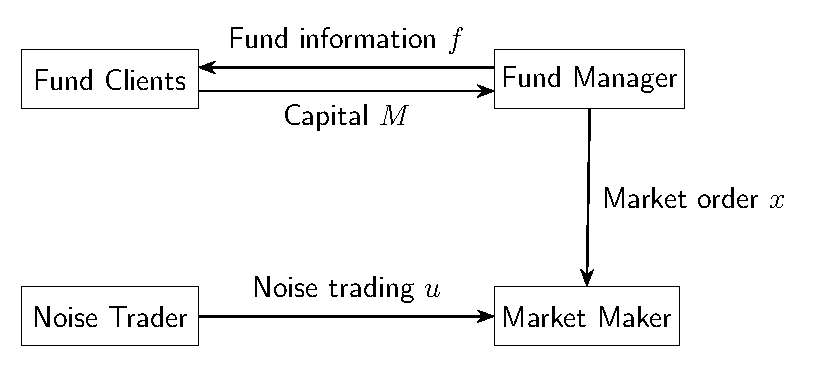
\includegraphics[width=0.65\linewidth]{./Figures/Fig_model.pdf}
\caption{Capital Allocation and Investment}\label{fig:model}
\end{figure}

We model the manager’s trading decision and investors' capital allocation as a simultaneous game with rational expectations, as illustrated in Figure \ref{fig:model}.

\paragraph{\normalfont{\it{Manager's tradign decision.}}}
Upon discovering the mispricing in the asset ($s$), the fund manager chooses the portfolio allocation between the risky and the safe asset. This action is represented by a market order for $x\in \mathbb{R}$ units of the risky asset, submitted to the market maker in the financial market. The manager decides on $x$ by incorporating the reactions of the financial market (i.e., the asset price) and the capital inflow from her investors, as described in the following.

\paragraph{\normalfont{\it{Investors' capital allocation.}}}
Each investor chooses the amount of capital to invest into the fund. Investor $i$'s capital allocation is denoted by $m_i \ge 0$, and the total fund flow or the asset under management (AUM) of the fund is defined by $M \equiv \sum_{i=1}^{n}m_{i}$. The fund’s fee structure is proportional to the total fund proceeds: the manager takes a $\phi\in(0,1)$ fraction of the proceeds, while the remaining $1-\phi$ fraction is distributed to the investors in proportion to their contributions to the fund, i.e., $m_i / M$.\footnote{Introducing a fixed fee does not change our qualitative results, as long as the performance-based fee also exists, $0 < \phi < 1$.}

\paragraph{\normalfont{\it{Financial market.}}}
In the financial market, the market maker sets the asset price, $p$, based on the incoming order flow, $x+u$, where $u$ represents a random market order from the noise trader and follows a normal distribution with mean zero and variance $\omega_u$. Due to competition, the market maker sets a semi-strong efficient price conditional on $x+u$:\footnote{Assume that, on the equilibrium path, one competitive market maker trades the asset. As in \citet{kyle1985continuous}, competitively many market makers exist off the equilibrium path, ensuring a break-even price in the equilibrium.} 
\begin{equation}
p=\mathrm{E}[\delta|x+u].\label{p}
\end{equation}


\subsubsection{Fund Opacity}
At the fund-raising stage, the manager disseminates a private noisy signal about her trading strategy to investors, defined as $f = x + e$, where $e$ represents a normally distributed noise term with mean zero and variance $\omega_{e}$.\footnote{We assume that $f$ is privately communicated between the manager and investors and is not observable to the market maker. Allowing the market maker to observe a noisy signal about $x$, however, does not affect the main qualitative results, as long as this signal differs from $f$, since the core results rely on the sensitivity of $p$ to $s$ being an increasing function of the manager's trading intensity.} This signal is referred to as the \textit{fund information}, and the noise variance of fund information, $\omega_e$, is used as the measure of \textit{fund opacity}. It describes the limited precision of the information that investors receive about the manager’s true trading strategy. A higher $\omega_{e}$ means that disclosed fund information is noisier, making the strategy harder to verify or reverse engineer. This reflects the idea that managers may deliberately obfuscate details by being vague, selective, or technically complex in their descriptions, while still engaging with investors to raise capital and to comply with disclosure rules.\footnote{For example, funds that largely track simple benchmark strategies are sometimes marketed using complex labels such as “dynamic opportunity,” “flexible growth,” or “adaptive allocation,” which convey sophistication while revealing little about actual portfolio construction. Similarly, managers may emphasize broad investment philosophies without clarifying how these translate into concrete portfolios.} Conversely, a lower $\omega_{e}$ corresponds to more transparent communication, allowing investors to form sharper beliefs about the manager’s actions.
Since the manager chooses her trading strategy $x$ based on the private signal $s$, the fund information $f$ is informative about the manager’s skill and the fund’s return. Thus, fund investors use $f$ to decide on their capital allocations. In what follows, we first consider the baseline model with exogenous opacity, while Section \ref{sec:endogenousopacity} endogenizes $\omega_{e}$ by allowing the manager to strategically choose fund opacity.

%\subsubsection{Misreporting and Verification.}
%\paragraph{\normalfont{\it{}}}
\subsubsection{Maximization Problems and Equilibrium}
The fund's profit from the risky investment is represented by $\pi\equiv(\delta-p)x$, so that the total fund proceeds, including those from the safe asset, are
\begin{equation}
    y=\pi+M.
\end{equation}
 %\paragraph{\normalfont{\it{Maximization problem.}}} 
Therefore, given the realized skill $s$, the fund manager maximizes her expected fee income by controlling her investment strategy $x$:
\begin{equation}
    \max_{x} \mathrm{E}\left[\phi y |s\right].\label{eq:managerproblem}
\end{equation}
Conversely, conditional on the fund information $f$, investor $i$ maximizes her expected return from delegating capital management:\footnote{The fund manager may have an incentive to make a false report about $y$ to her investors. Namely, by reporting $\tilde{y}$, she pays out $(1-\phi)\tilde{y}$ to investors and captures $y-(1-\phi)\tilde{y}$ on her own. To prevent this intentional misreporting, we assume that each investor can verify $x$ after the trading stage. Alternatively, we may assume costly verification: investors collectively pay the verification cost $C$ to back out $x$ from the fund information in the end of the trading period. As long as $C$ positively depends on the degree of fund opacity $\omega_e$, our qualitative results remain the same.}
\begin{equation}
    \max_{m_i\ge 0}\mathrm{E}\left[\frac{m_i}{M}(1-\phi)y -m_{i}|f\right].\label{eq:investorproblem}
\end{equation}
Note that the first term represents the expected payment from the fund, and the second term is the cost of capital.

\begin{definition}\label{def:eqm}
    The equilibrium is defined by the market maker's pricing strategy $p$, the fund manager's trading strategy $x$, and investors' capital allocations $\{m_{i}\}_{i=1}^{n}$, such that, (i) $p$ satisfies \eqref{p} given $x+u$, (ii) $x$ solves (\ref{eq:managerproblem}) given $s$, $p$, and $\{m_{i}\}_{i=1}^{n}$, and (iii) for all $i$, $m_i$ solves (\ref{eq:investorproblem}) given $p$, $f$, and $\{m_j\}_{j\neq i}$.

\end{definition} 
%*==*==*==*==*==*==*==*==*==*==*==*==*==*==*
\section{Equilibrium} \label{sec:eqm}
In this section, we search for a linear equilibrium in which the manager's market order $x$ is linear in her skill $s$, and the market maker's pricing strategy $p$ is also linear in the order flow $x+u$. Proofs for the analytical results are provided in the \hyperref[app:appendix]{Appendix}.

%===========================================
\subsection{Trading Strategy} \label{ss:conjecture}
Conjecture and later verify that the manager's equilibrium trading strategy is
\begin{equation}
 x(s)=\beta s,\label{x_conj}
\end{equation}
where $\beta>0$ is an endogenous constant determined in the equilibrium. Conjecture \eqref{x_conj} states that the manager buys (sells) the asset if her $s$ is positive (negative), where the order size is proportional to her skill $|s|$; the more skilled the manager, the more aggressively she trades.\footnote{This conjecture follows from the original Kyle model where an informed trader trades based on the difference between her belief and that of the market maker, i.e., $ \mathrm{E}[\delta|s]-\mathrm{E}[\delta] = s$.} The scale factor $\beta$ is referred to as the {\it trading intensity}, representing how intensively the manager exploits her informational advantage over the market maker.

%===========================================
\subsection{Execution Price} \label{ss:price}
The market maker decides on the price of the asset by extracting information about the asset's payoff from the aggregate order flow $x+u$. Anticipating the trading strategy \eqref{x_conj}, the price in equation \eqref{p} can be rewritten as
\begin{equation}
p=\bar{\delta}+\lambda(x+u),\label{eq:p}
\end{equation}
where
\begin{equation}
\lambda\equiv \frac{\beta \omega_{s}}{\beta^{2} \omega_{s}+\omega_{u}}\label{lambda}
\end{equation}
is referred to as ``Kyle's lambda,'' a measure of the price impact of order flow.\footnote{Since the market maker believes that the manager follows \eqref{x_conj}, the linear filtering rule with normally distributed random variables yields $p=\mathrm{E}[\bar{\delta} + s|\beta s + u] = \bar{\delta}+\mathrm{E}[s]+\frac{\mathrm{Cov}[s,\beta s+u]}{\mathrm{Var}[\beta s+u]}(x+u-\mathrm{E}[\beta s+u])=\bar{\delta}+\frac{\beta \omega_{s}}{\beta^{2} \omega_{s}+\omega_{u}}(x+u)$.} Following the literature, we define a market to be {\it liquid} if $\lambda$ is small.
%\footnote{From \eqref{p}, we have $p=\mathrm{E}[\delta|x+u]=\mathrm{E}[\mathrm{E}[\delta|x+u,s]|x+u]=\mathrm{E}[\bar{\delta}+s|x+u]$. Since the market maker believes that the manager follows \eqref{x_conj}, $s$ and $x+u$ are both normally distributed from the market maker's perspective. Thus, $p=\bar{\delta}+\mathrm{E}[s]+\frac{\mathrm{Cov}[s,x+u]}{\mathrm{Var}[x+u]}(x+u-\mathrm{E}[x+u])=\bar{\delta}+\frac{\mathrm{Cov}[s,\beta s+u]}{\mathrm{Var}[\beta s+u]}(x+u-\mathrm{E}[\beta s+u])=\bar{\delta}+\frac{\beta \omega_{s}}{\beta^{2} \omega_{s}+\omega_{u}}(x+u)$.}
%===========================================
\subsection{Investors' Capital Allocation} \label{ss:delegation}
By incorporating the fund proceeds $y = \pi + M$, investor $i$'s optimization problem in (\ref{eq:investorproblem}) is 
\begin{equation}
    \max_{m_i\ge 0} \frac{m_i}{M}(1-\phi)\mathrm{E}\left[\pi|f\right]-\phi m_i.\label{eq:mi_max}
\end{equation}
Investor $i$ solves this problem by incorporating the impact of her choice ($m_i$) on the total fund flow ($M$), while taking other investors' behavior ($\sum_{j\neq i} m_j$) as given. As she allocates a larger amount of capital, its marginal return diminishes due to the pro-rata allocation of the fund's proceeds, while the cost of capital linearly increases. This structure ensures the second-order condition of problem \eqref{eq:mi_max}, and the first-order condition pins down the optimal capital allocation as follows:
\begin{equation}
    m_{i}= \left(\frac{1-\phi}{\phi}\mathrm{E}[\pi|f]\sum_{j\neq i}m_j\right)^{\frac{1}{2}} -\sum_{j\neq i}m_j.
    \label{eq:mi}
\end{equation}
We focus on the symmetric equilibrium where all investors take the same action, $m_i = m$ for all $i=1,2,\cdots,n$. In this equilibrium, equation \eqref{eq:mi} reduces to 
\begin{equation}
    m = \frac{n-1}{n^2}\frac{1-\phi}{\phi}\mathrm{E}[\pi|f],\label{eq:m_sym}
\end{equation}
and the total fund flow becomes
\begin{equation}
    M \equiv n m = \theta \mathrm{E}[\pi|f],\label{eq:M_sym}
\end{equation}
where $\theta \equiv \frac{n-1}{n}\frac{1-\phi}{\phi}$ represents the \textit{flow-performance sensitivity}.  
Both the individual capital allocation and the total fund flow are linearly increasing in the expected trading profit conditional on the fund information, $\mathrm{E}[\pi|f]$. This is due to the performance-based fee structure, which makes the per-unit return from delegated asset management increasing in the trading profit. Also, equation (\ref{eq:M_sym}) specifies the flow-performance sensitivity $\theta$, which governs the reaction of the fund flow to the expected fund performance. The fund flow becomes less sensitive to the expected performance when the fee rate ($\phi$) is high, as high $\phi$ raises the cost of delegation and discourages investment, while it becomes more sensitive when the fund has a large clientele ($n$), as it attracts capital from a larger number of  investors.

\subsection{Reputation}
In determining the capital callocation in \eqref{eq:m_sym}, each investor seeks to compute the expected fund profits $\mathrm{E}[\pi|f]$. This process, in turn, requires the investor to back out the realized skill level of the manager $|s|$ from fund information $f=x+e$. 

% When the fund information is perfectly transparent (i.e., $\omega_{e}=0$), investors rationally use the trading strategy in \eqref{x_conj} and infer $s = x/\beta$, leading to\footnote{Given the linear pricing rule in \eqref{eq:p}, it holds that $\pi = (\delta - p)x = (s-\lambda \beta x)x$. Adopting trading strategy $x=\beta s$ leads to equation \eqref{eq:exp_pi_transparent}.}
% \begin{equation}
%       \mathrm{E}\left[\pi|f\right] = (1-\lambda \beta)\beta\mathrm{E}[s^2|s=x/\beta]=\left(\frac{1}{\beta}-\lambda\right)x^2.\label{eq:exp_pi_transparent}
% \end{equation}
% The first equality in (\ref{eq:exp_pi_transparent}) suggests that the fund return, $\pi=(\delta-p)x$, becomes a quadratic function of $s$, as both the manager's trading quantity $x$ and the profit margin, $\delta-p$, are proportional to the skill level in expectation. Furtheremore, the transparent fund information indicates that $s=x/\beta$, thereby shaping the conditional expected profit into quadratic in $x$, as the second equality in \eqref{eq:exp_pi_transparent} attests. 

% %This result implies that, on top of the maximizing profits, delegated asset management generates an additional incentive for the manager to control her trading strategy $x$, as it affects the total fund flow $M$ by influencing the investors' expectation about fund's returns.





% %===========================================
% \subsection{Manager's Optimization} \label{ss:optimization}
% By incorporating the total fund flow ([\ref{eq:M}] and [\ref{eq:exp_pi_transparent}]), the manager's problem in (\ref{eq:managerproblem}) is re-written as
% \begin{equation}
%     \max_{x} \phi\left(sx - \lambda x^2   + \theta\left(\frac{1}{\beta}-\lambda\right)x^2\right).\label{eq:managerproblem_transparent}
% \end{equation}
% The first two terms represent the fee income from the trading profit and are essentially identical to the trading profit in the original \citet{kyle1985continuous} model. The third term arises due to the fund inflow and, as equation (\ref{eq:exp_pi_transparent}) demonstrates, is determined by the quadratic size of risky investments. The optimal trading strategy solves \eqref{eq:managerproblem_transparent}, leading to
% \begin{equation}
%     x = \frac{1}{2}\frac{\beta}{\lambda\beta - \theta(1-\lambda\beta)}s.\label{eq:x=Fbeta}
% \end{equation}
% It is consistent with our guess in (\ref{x_conj}) when: 
% \begin{equation}
%     \beta = \frac{1}{2}\frac{\beta}{\lambda\beta - \theta(1-\lambda\beta)}.\label{eq:fixedpoint-transparent}
% \end{equation}
% By solving $\lambda$ and $\beta$ in equations (\ref{lambda}) and \eqref{eq:fixedpoint-transparent}, the trading strategy and the asset price are uniquely determined:
% \begin{lemma}\label{lem:transparent}
%     When the fund information is transparent ($\omega_{e}=0$), the manager's trading strategy and the asset price are specified by \eqref{x_conj} and \eqref{eq:p} with 
%     \begin{equation}
%         \beta = \sqrt{(1+2\theta)\frac{\omega_{u}}{\omega_{s}}},\label{eq:eqm_trade_transparent}
%     \end{equation}
%     and
%     \begin{equation}
%         \lambda = \frac{1}{2(1+\theta)}\sqrt{(1+2\theta)\frac{\omega_{s}}{\omega_{u}}}.\label{eq:eqm_lambda_transparent}
%     \end{equation}
% \end{lemma}
% %As is evident from problem (\ref{eq:managerproblem_transparent}), the flow-performance sensitivity, $\theta$, captures the manager's additional incentive to inflate her risky investment. 
% In the absence of delegated asset management ($\theta\rightarrow0$), the equilibrium is identical to the original \citet{kyle1985continuous} model, where $\beta$ is determined to maximize the expected trading profits. On one hand, the manager seeks to exploit her informational advantage by trading more intensively. On the other hand, it reveals information to the market maker and raises the price impact, cutting into the trading profit. The equilibrium $\beta$ balances these competing effects.

% Delegated asset management ($\theta>0$) brings about the additional risk-taking incentive, because inflating $x$ benefits the manager by making her appear highly skilled and inducing a larger fund flow (see equations [\ref{eq:M}] and [\ref{eq:exp_pi_transparent}]). We refer to this incentive as the ``showing-off'' motive. Since $\theta$ governs the flow-performance sensitivity, this motivation becomes stronger when $\theta$ is large, shaping equilibrium $\beta$ into an increasing function of $\theta$.

% Equation \eqref{eq:eqm_lambda_transparent} shows that the price impact $\lambda$ decreases with $\theta$. This is because the information is exaggerated in that the order size is too large relative to the true $|s|$ due to the showing-off motive. Thus, the market maker attempts to partially undo the manager's information revelation by incorporating less of it into the price, resulting in a weaker price impact.\footnotemark
% \footnotetext{\label{fn:footnote}$\lambda$ represents the price's reaction to the order flow $x+u$, rather than its reaction to the manager's private information $s$. The price impounds $s$ with coefficient $\beta\lambda$, which is monotonically increasing in $\theta$.}

% Our benchmark result in Lemma \ref{lem:transparent} isolates the fundamental mechanism through which delegated asset management enhances the manager’s risk taking behavior. The tendency of fund managers to show off their skill to attract capital is well discussed in the literature (e.g., \citealp{metrick2010economics}; \citealp*{chung2012pay}; \citealp{barber2017interim}), raising regulatory concerns that fund managers have incentives to exaggerate the performance or quality of their funds. In our model, however, a skilled manager may also have incentives to conceal her skill from the market maker, as emphasized by \citet{kyle1985continuous}. The next section explores how the fundamental tension between the showing off and the hiding motives shapes the equilibrium when the fund information becomes harder to interpret for investors due to opacity.
\section{Opaque Funds} \label{sec:endogenous}
This section introduces the fund opacity, $\omega_{s}>0$, and demonstrates that belief-driven mltiple equilibria show up regarding the trading strategy of the fund. We discuss economic implications drawn from the equilibrium analyses in Subsection \ref{ss:implications}.

%===========================================
\subsection{Delegation under Fund Opacity}\label{subsec:opaquedelegate}
Assuming that $\omega_{s}>0$, the analysis of an opaque fund largely follows the benchmark case in Section \ref{sec:Model}. In particular, investors' optimization and the structure of the resulting fund flow are identical to those in (\ref{eq:symmetricm}) and (\ref{eq:M}) in the benchmark model. However, due to the noisy revelation of the fund information, investors' conditional expectation about the fund return must be modified as follows:

\begin{lemma}\label{lem:reputation}
	Upon observing the fund information, $x+e$, investors' updated expected trading profit is given by
	\begin{equation}
         \mathrm{E}\left[\pi|x+e\right] = (1-\lambda \beta)\beta\left(\hat{s}^2 + \hat{\omega}_{s}\right),
     \end{equation}
     where the posterior expectation of the (signed) realized skill is
     \begin{equation}
         \hat{s} = \mathrm{E}[s|x+e] = \xi(x+e),
     \end{equation}
     with 
	 \begin{equation}
		\xi = \frac{\beta\omega_{s}}{\beta^2 \omega_{s}+\omega_{e}},\label{eq:xi}
	 \end{equation}
	 and the posterior of the skill variance is
     \begin{equation}
         \hat{\omega}_{s} = \mathrm{Var}[s|x+e] = \frac{\omega_{s}\omega_{e}}{\beta^2 \omega_{s} + \omega_{e}}.
     \end{equation}
 \end{lemma}
 Investors update their belief about the realized skill using $x+e$, where $\xi$ measures how much they rely on the fund information provided by the manager. Holding $\beta$ constant, $\xi$ is large when investors' prior is unreliable ($\omega_{s}$ is large) and the fund information is transparent ($\omega_{e}$ is small). In what follows, the updated expectation about the manager's realized skill, $\hat{s}$, is referred to as the \textit{reputation}.  

 \subsection{Manager's Optimization} \label{ss:optimization_opaque}
Following the same procedures as the transparent benchmark, the manager's optimization problem in (\ref{eq:managerproblem_transparent}) is re-written as follows:
\begin{equation}
	\max_{x}\ sx - \lambda x^2 + \theta(1-\lambda\beta)\beta \left[\xi^2(x^2 + \omega_{e}) + \hat{\omega}_{s}\right].\label{eq:managerproblem opaque}
\end{equation}
As in the baseline model, the first two terms of equation (\ref{eq:managerproblem opaque}) represent the trader's expected trading profit. The third term corresponds to her profits from the fund flow, $M$, which also increases with $|x|$ because she can potentially inflate her reputation $|\hat{s}|$ by placing a large order (either buy or sell).

The unique solution to \eqref{eq:managerproblem opaque} (given $\beta$) is
\begin{equation}
x=F(\beta)s,\label{x}
\end{equation}
where
\begin{equation}
F(\beta)\equiv\frac{1}{2\left(\lambda-\theta(1-\lambda\beta)\beta\xi^{2}\right)}.\label{F}
\end{equation}
$F(\cdot)$ is a nonlinear in $\beta$ because $\lambda$ and $\xi$ are functions of $\beta$. 

%===========================================
\subsection{Equilibrium under Opacity} \label{ss:equilibrium}
The manager optimally chooses \eqref{x} given that the market maker and investors believe that she follows strategy \eqref{x_conj}. In equilibrium, their beliefs must be correct, that is, \eqref{x_conj} and \eqref{x} must be consistent with each other, requiring the following condition:
\begin{equation}
\beta=F(\beta).\label{fixed_point}
\end{equation}
That is, the equilibrium levels of $\beta$ are determined at the fixed points of $F(\cdot)$. Having identified $\beta$, the equilibrium levels of $x$, $p$, and $m$ are determined by equations \eqref{x_conj}, \eqref{eq:p} and \eqref{eq:symmetricm}, respectively. In what follows, we first illustrate the determination of equilibrium $\beta$ through a numerical example, followed by an analytical proposition that formally establishes the equilibria.


\begin{figure}
\centering
\subfigure[Small $\theta$ ($\theta=0.2$) $\Rightarrow$ unique low-$\beta$ equilibrium.]{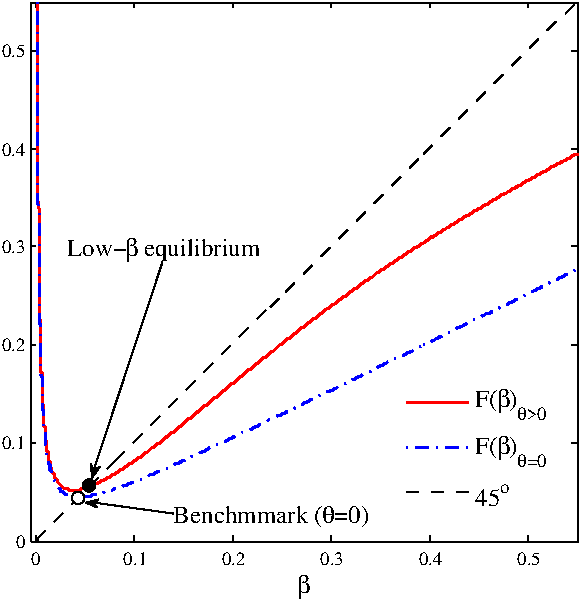
\includegraphics[width=67mm]{./Figures/fig_exogenous_low.pdf}
\label{low}}\quad
\subfigure [Large $\theta$ ($\theta=0.55$) $\Rightarrow$ unique high-$\beta$ equilibrium.]{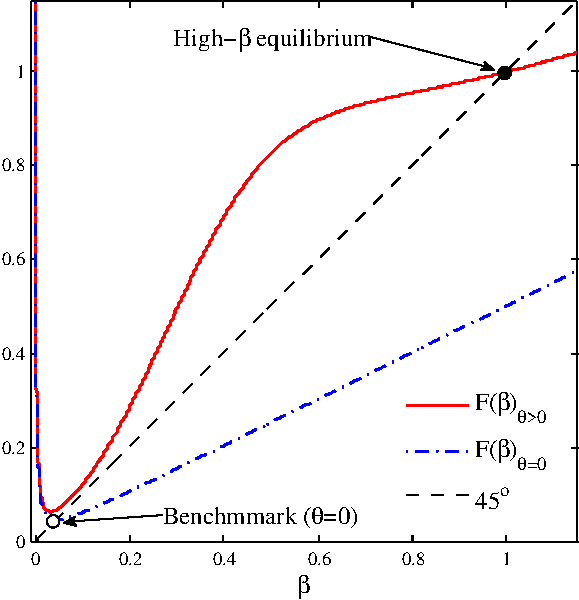
\includegraphics[width=67mm]{./Figures/fig_exogenous_high.pdf}\label{high}}\\[15pt]
\subfigure[Intermediate $\theta$ ($\theta=0.33$) $\Rightarrow$ multiple high-$\beta$ \& low-$\beta$ equilibria.]{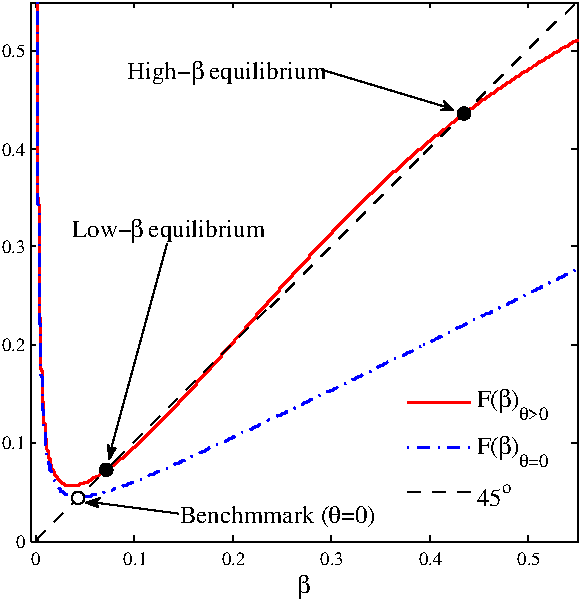
\includegraphics[width=67mm]{./Figures/fig_exogenous_multiple.pdf}\label{multi}}\\[10pt]
\caption{Determination of $\beta$}
\caption*{\footnotesize{Note: The figure plots $F(\beta)$ for different values of $\theta$. The equilibrium values of $\beta$ are determined at the fixed points of $F(\cdot)$.  The parameter values used in the figures are $\omega_{s}=50$, $\omega_{\delta}=1$, and $\omega_{u}=0.1$.}}
\label{fig:exog}
\end{figure}


Figure \ref{fig:exog} illustrates the determination of $\beta$ for three different levels of fund opacity, $\omega_{e}$.
%\footnote{In Figure \ref{fig:exog}, $\omega_{s}$ is assumed to be relatively large. As Proposition \ref{prop:eqm} below formalizes, if $\omega_{s}$ is sufficiently small we do not obtain multiple equilibria as in panel (c) of Figure \ref{fig:exog}.} 
The intersections of $F(\beta)$ (the solid line) and the 45-degree line yield the equilibrium levels of $\beta$. We also plot $F(\beta)$ with $\theta=0$ (the dash-dotted line) and denote its solution as $\beta_{\theta=0}$ to highlight the original model of \citet{kyle1985continuous} where fund delegation is irrelevant.

Panel (a) of Figure \ref{fig:exog} shows that if $\omega_{e}$ is large, there is a unique ``low-$\beta$ equilibrium'' where $\beta$ is close to $\beta_{\theta=0}$. Panel (b) shows that a large $\omega_{e}$ leads to a unique ``high-$\beta$ equilibrium,'' in which $\beta$ is much larger than $\beta_{\theta=0}$.
%\footnote{Formally, we define an equilibrium to be low-$\beta$ (high-$\beta$) if $\beta<\tilde{\beta}$ ($\beta>\tilde{\beta}$), where $\tilde{\beta}$ is defined as square root of the unique solution to equation (\ref{eq:T}) in Lemma \ref{lem:K(1)K(2)} of Online Appendix \ref{proofendogenous}. In the context of Figure \ref{fig:exog}, a low-$\beta$ equilibrium is given by a fixed point of function $F$ at which $F$ is convex and U-shaped, while a high-$\beta$ equilibrium is given by a fixed point that is larger than the first inflection point of $F$. Using this definition, Kyle’s original equilibrium ($\theta=0$) is classified as a low-$\beta$ equilibrium.\label{fn:highlowbeta_def}}
Panel (c) shows that multiple equilibria arise for an intermediate level of $\omega_{e}$. Specifically, the high-$\beta$ and the low-$\beta$ equilibria are stable, as $F(\beta)$ crosses the 45-degree line from above, whereas the one with an intermediate $\beta$ is unstable, as $F(\beta)$ crosses the line from below.\footnote{We define an equilibrium to be stable (unstable) if the corresponding $\beta$ is a stable (unstable) fixed point of $F(\cdot)$, that is, $|F^{\prime}(\beta)|<1$ $(>1)$. A stable equilibrium is robust to a small perturbation to the agents' belief about $\beta$, meaning that the economy converges back to the original equilibrium through the best-response dynamics of the agents' beliefs.}  In what follows, we focus only on the stable equilibria. 

%Panel (a) of Figure \ref{fig:exog} shows that if the trader's reputation concern is weak (i.e., $\theta$ is small), the reputation-driven equilibrium vanishes and only the one close to the benchmark is supported (panel (b)). If the reputation concern is very strong, the Kyle-like equilibrium vanishes and only the one far from the benchmark holds (panel (c)). Multiple equilibria arise if, and only if, the degree of reputation concerns is intermediate (panel (a)). 

\paragraph{\normalfont{\it{Impact of fund opacity.}}}

To see the intuition behind the different equilibrium patterns presented in Figure \ref{fig:exog}, note that the fund manager faces two conflicting motives when trading. On the one hand, she seeks to avoid trading too aggressively on her private information, as doing so would move the price excessively and reduce her trading profits. As in \citet{kyle1985continuous}, this motive leads the trader to decrease $\beta$. On the other hand, she wishes to trade intensively to signal her high skill to her client investors, aiming to establish a strong reputation and attract a large fund flow. This motive encourages her to increase $\beta$. In summary, she faces a tradeoff between ``hiding'' her skill from the market maker and ``showing it off'' to her clients. The fund opacity, $\omega_{e}$, governs this tradeoff by influencing the sensitivity of the manager's reputation, $\hat{s}$, to her investment behavior, $x$. In particular, Lemma \ref{lem:reputation} demonstrates that the fund flow becomes insensitive to $x$ under opacity, as it becomes difficult for investors to estimate the skill based on the fund information, weakening the showing-off motive.

For a opaque fund with a large $\omega_{e}$ (panel (a)), the hiding motive dominates the showing-off motive, leading to a unique low-$\beta$ equilibrium. In this equilibrium, client investors believe that the manager's trading intensity is relatively low. Knowing this, the manager could inflate her reputation by placing an order larger than what her clients anticipates. However, she would refrain from doing so because it would cause a large price impact, reducing the fund's investment profits. Consequently, the equilibrium $\beta$ is close to $\beta_{\theta=0}$, meaning that it is a ``Kyle-like equilibrium." 

For a transparent fund with a small $\omega_{e}$ (panel (b)), the showing-off motive prevails, resulting in a unique high-$\beta$ equilibrium. In this equilibrium, the manager is willing to move the price substantially, undermining investment profits to appear skilled. Importantly, client investors' learning is not manipulated, as their belief about the manager's trading strategy is correct. Nonetheless, the manager places a large order because doing otherwise would induce her clients to incorrectly estimate that she is less skilled, thereby deteriorating her reputation. She trades aggressively solely to conform to her clients' belief. To emphasize this mechanism, we call this equilibrium the ``reputation-driven equilibrium."

For intermediate levels of $\omega_{e}$ (panel (c)), there is no clear dominance between the two motives, hence both the low-$\beta$ and the high-$\beta$ equilibria are supported under intermediate fund opacity. Each equilibrium is associated with a self-fulfilling belief of the market maker and investors.

The following proposition and Figure {\ref{fig:theta}} summarize the above discussion and provide an analytical characterization of the equilibria.

\begin{figure}[t]
    \centering
    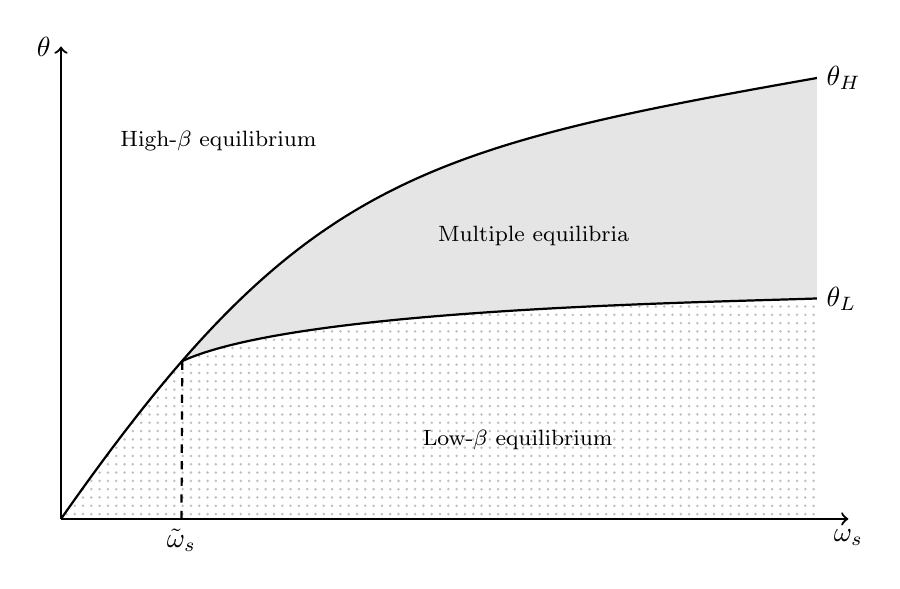
\begin{tikzpicture}[scale=2.0]

    % Axes
    \draw[thick,->] (0,0) -- (5,0) node[below] {$\omega_{s}$};
    \draw[thick,->] (0,0) -- (0,3) node[left] {$\theta$};
    % Fill below theta_L and right of threshold with dots
    \fill[pattern=dots, pattern color = black!25] 
        (0,0) to [out = 55, in = 190, looseness=1.2](4.8,2.8)
        -- (4.8, 0)
        to (0,0)
        -- cycle;
    % Fill by gray
    \fill[gray!20] 
        (0.765,1.) to [out = 25, in = 182, looseness=0.5](4.8,1.4)
        -- (4.8,2.8)
        to [out = 190, in = 49, looseness=1.02] (0.765,1.)
        -- cycle;
    % Curves
    %\draw[thick, blue, domain=0:4.8, samples=300] plot (\x, {0.08*(-(\x)^2 + 12*(\x)}) node[right] {$y = x^{0.3}$};
    \draw[thick] (0,0) to [out = 55, in = 190, looseness=1.2](4.8,2.8);
    \draw[thick] (0.765,1.) to [out = 25, in = 182, looseness=0.5](4.8,1.4);
    
    
    
    

    

        
    % Labels
    \node at (1.0,2.4) {\footnotesize High-$\beta$ equilibrium};
    \node at (3,1.8) {\footnotesize Multiple equilibria};
    \node at (2.9, 0.5) {\footnotesize Low-$\beta$ equilibrium};
    

    % Points at the end of curves
    \node[right] at (4.8,2.8) {$\theta_H$};
    \node[right] at (4.8,1.4) {$\theta_L$};

    % Threshold for multiple eqm
    \draw[thick,dashed] (0.77,1.) -- (0.765,0) node[below] {$\tilde{\omega}_{s}$};

    \end{tikzpicture}
    \caption{Equilibrium Characterization with Exogenous $\theta$}
    \caption*{\footnotesize{Note: This figure illustrates the equilibrium states using the reputation concern, $\theta$, and the skill potential, $\omega_{s}$.}}
    \label{fig:theta}
\end{figure}

\begin{proposition}[Equilibrium characterization]\label{prop:eqm}
There exists a critical value of the fund opacity, $\tilde{\omega}_{e}=8\omega_{u}$, and two thresholds of the flow-performance sensitivity, $\theta_{L}$ and $\theta_{H}$ ($\ge \theta_{L}$), such that,
\begin{enumerate}[label=(\roman*)]
	\item if $\omega_{e}\leq \tilde{\omega}_{e}$, then $\theta_{L}=\theta_{H}=\theta_{0}$, and the low-$\beta$ equilibrium uniquely arises when $\theta<\theta_{0}$, while the high-$\beta$ equilibrium uniquely arises when $\theta>\theta_{0}$; and 
	\item if $\omega_{e}> \tilde{\omega}_{e}$, then $\theta_{H}>\theta_{L}$. $\theta> \theta_{H}$ leads to a unique high-$\beta$ equilibrium, $\theta\leq\theta_{L}$ leads to a unique low-$\beta$ equilibrium, and $\theta\in(\theta_{L},\theta_{H})$ leads to multiple equilibria.
\end{enumerate}
\end{proposition}

%Together with the fund opacity, $\omega_{e}$, the flow-performance sensitivity, $\theta$, also influences the equilibrium characterization, as it determines the importance of the fund inflow and thus the reputation in the manager's utility. Proposition \ref{prop:eqm} demonstrates that combinations of a sufficiently opaque fund ($\omega_{e}>\tilde{\omega}_{e}$) and intermediate values of flow-performance sensitivity ($\theta_{L}<\theta<\theta_{H}$) bring about multiple equilibria. As explained earlier, opacity leads to the manager's conflicting motives to trade intensively. When $\theta$ is intermediate, the fund flow is moderately significant in the manager's utility, thereby eliminating a clear dominant strategy for the manager.
\paragraph{\normalfont{\it{Impact of flow-performance sensitivity.}}}
Proposition \ref{prop:eqm} and Figure \ref{fig:theta} indicate that, for a given fund opacity, $\omega_{e}$, a weak flow-performance sensitivity supports only the low-$\beta$ equilibrium, while increases in $\theta$ can generate the high-$\beta$ equilibrium, potentially leading to multiple equilibria.\footnote{Lemma \ref{lem:theta_s} in Online Appendix \ref{proofendogenous} analytically characterizes the upward-sloping $\theta_{H}$ and $\theta_{L}$ in relation to $\omega_{e}$, as presented in Figure \ref{fig:theta}.} To understand intuition, the tradeoff between hiding and showing-off motives, as explained above, is key. 
%On the one hand, she seeks to avoid trading too aggressively on her private information, as doing so would move the price excessively and reduce her trading profits. On the other hand, she wishes to trade intensively to show off her skill to the recruiter. 
When $\theta$ is small, the fund flow's reaction to changes in the expected investment profit becomes weak. In this case, the manager’s showing-off motive is less important. Consequently, the hiding motive prevails, prompting her to trade less aggressively and leading to the low-$\beta$ equilibrium. Conversely, when $\theta$ is large, the fund flow becomes highly sensitive to the fund information, thereby encouraging the manager to show off her skill by trading intensively. This scenario gives birth to the high-$\beta$ equilibrium.

Overall, the type of equilibrium depends on the combination of $\theta$ and $\omega_{e}$, as illustrated in Figure \ref{fig:theta}. The tradeoff between the hiding and the showing-off motive tends to balance and generates multiple equilibria when the fund is relatively opaque, and the fund flow is moderately sensitive to the expected investment performance. Otherwise, one of the conflicting motives dominates the other either because of a sufficiently transparent fund, encouraging the manager to show off her skill, or the fund flow being very sensitive or insensitive to the expected performance, altering the importance of the fund flow relative to the investment profit in the manager's optimization.

\paragraph{\normalfont{\it{Equilibrium comparison.}}}
Comparing the two stable equilibria, does the manager perform better in one of them? What are the implications for market liquidity, asset prices, and learning about asset-selection skills? 
%The following corollary summarizes the results.
\begin{corollary}[High-$\beta$ vs.\ low-$\beta$ equilibrium]\label{cor:high_vs_low}
In the high-$\beta$ equilibrium, relative to the low-$\beta$ equilibrium,
\begin{enumerate}[label=(\roman*)]
\item \label{item:1} the market liquidity is higher, that is, $\lambda$ is lower;
\item \label{item:2} the manager's expected trading profit given the realized skill, $\mathrm{E}[(\delta-p)x|s]=\frac{\beta\omega_{u}s^{2}}{\beta^{2} \omega_{s}+\omega_{u}}$, is lower;
\item \label{item:3} the price informativeness, $\tau\equiv\frac{1}{\mathrm{Var}[\delta|p]}=\frac{\beta^{2} \omega_{s}+\omega_{u}}{\omega_{\delta}(\beta^{2} \omega_{s}+\omega_{u})+\omega_{u} \omega_{s}}$, is higher;
\item \label{item:4} the price volatility, $\mathrm{Var}[p]=\frac{\beta^{2}\omega_{s}^{2}}{\beta^{2} \omega_{s}+\omega_{u}}$, is higher; and
\item \label{item:5} investors' estimate of $s$ is more precise, that is, the posterior variance of $s$, $\hat{\omega}_{s}=\frac{\omega_{s}\omega_{u}\omega_{\delta}}{\omega_{s}(\beta^{2}\omega_{\delta}+\omega_{u})+\omega_{u}\omega_{\delta}}$, is lower.
\end{enumerate}
\end{corollary}

Statement \ref{item:1} of Corollary \ref{cor:high_vs_low} holds because price impact $\lambda$ is decreasing in $\beta$ in the equilibrium. Since the high-$\beta$ equilibrium emerges only if $\theta$ is relatively large, the statement also implies that a higher flow-performance sensitivity leads to higher market liquidity. The intuition is as follows. Relative to the low-$\beta$ equilibrium, in the high-$\beta$ equilibrium the manager trades more aggressively, and thus the order flow reflects significant information about $s$. To incorporate the appropriate amount of information about $s$ into the price, the market maker seeks to offset the exaggerated information in order flow by lowering $\lambda$.

The intuition for statement \ref{item:2} is closely related to that for statement \ref{item:1}. In the high-$\beta$ equilibrium, the manager earns a lower trading profit due to a smaller informational advantage over the market maker. This result may appear inconsistent with statement \ref{item:1} because, ceteris paribus, a lower price impact is typically associated with a higher trading profit. However, the manager's order size $|x|$ in the high-$\beta$ equilibrium is so large that the {\it overall} price impact (i.e., $\lambda$ multiplied by $|x|$) is larger than that in the low-$\beta$ equilibrium. Consequently, the manager moves the price excessively and earns a lower trading profit in this equilibrium.
%\footnote{Our numerical result, not presented in the paper but available upon request, indicates that the trader's overall expected utility, including the reputation benefit, is also lower in the high-$\beta$ equilibrium.} 
Due to her aggressive trading, more information about $s$---which is informative about $\delta$---is incorporated into the price in the high-$\beta$ equilibrium, supporting statement \ref{item:3}.

Statement \ref{item:4} follows, again, from the manager's aggressive trading in the high-$\beta$ equilibrium. Specifically, she places a large buy (sell) order when $s>0$ ($s<0$), even if $|s|$ is small. This causes a large upward (downward) pressure on $p$, leading to greater price variability. This result aligns with the insight of \citet{guerrieri2012fund} that reputation concerns amplify price volatility, although their mechanism differs from ours.\footnote{\citet{guerrieri2012fund} argue that bond price volatility increases because fund managers demand a premium to offset the risk of reputation damage in the event of default.}

In the high-$\beta$ equilibrium, the manager reveals more information about $s$, thereby improving the precision of investors' estimation (statement \ref{item:5}). This makes the fund flows more responsive to skill, as investors can assess it more accurately.

%{\color{red} [TO ADD, perhaps, what our model would imply about increasing skill ($\sigma_{s}^2$), an increasing industry, and no improvement in aggregate performance.]}

%{\color{red}[TO ADD HERE, MAYBE: Learning in our model is not based on performance as measured by profits. We have many sources of info, price and payoff, return... but it's not return on its own... it's important for the incentive to move the price]}


%%-------------------------------------------
%\subsubsection{No noise trading}
%Our model also yields a result that is intriguing from a somewhat technical point of view: reputation-driven trades occur even if we do not assume noise traders.
%\begin{corollary}[No noise trading]\label{cor:no_noise_trading}
%Even in the absence of noise traders (i.e., $\sigma_{u}=0$), each trader trades in a stable equilibrium if $\theta>0$. She submits $x=2\thetas$ while the price $p=\hat{\delta}+s$ fully reveals her $s$, and her expected trading profit is $\mathrm{E}[\pi|s]=0$.
%\end{corollary}
%This result contrasts with Kyle (1985) and many other finance models in which trades occur only at the expense of noise traders. In these models, a trader would submit $x=0$ and therefore the market would break down if $\sigma_{u}=0$. The absence of noise traders implies that the market maker knows the exact level of $x$, which fully reveals the trader's information. This is the reason $x=0$ would hold if $\sigma_{u}=0$ in Kyle (1985).\footnote{To see why $x=0$ holds, consider what would happen to our equilibrium if $\theta=0$. Suppose that the market maker believes $x=\betas$ for some $\beta>0$. Then, from \eqref{x}, the trader's best response is to choose $x=F(\beta)s=\frac{1}{2\lambda}s=\frac{\beta}{2}s$. That is, she trades less aggressively than the market maker's belief. She does so in an effort to lead the market maker to underestimate $|s|$ so she can exploit the resulting mispricing. But the market maker would rationally anticipate it. So, suppose that the market maker believes  $x=\frac{\beta}{2}s$. Then the trader's best response is to choose $x=\frac{\beta}{4}s$ for the same reason as above. Continuing this way, the only situation supported as an equilibrium is that the trader chooses $x=0$ and the market maker correctly believes it.} But in our model, the trader chooses $x\neq 0$ due to the reputation concern: if, for whatever reason, the recruiter believes that $\beta>0$, the trader needs to conform with it and submit $x\neq 0$, since otherwise the recruiter would believe ex post that $|s|=0$, leading to zero reputation benefit. She does so while knowing that such a trade will make zero expected profit.

%Our numerical exercises suggest that the trader's unconditional expected utility is higher in the low equilibrium. While the expected reputation gain is increasing in $\beta$, the increase is not high enough to make up for the decrease in profits. We obtain similar results conditional on skill, with the exception that for low skill, $|s|$, trading more aggressively lowers both the expected profit and the expected reputation gain. 

%\subsubsection{Comparative statics} \label{sss:compStat}
%%-------------------------------------------------------------------------------------------------------------------
%[\textbf{Two period model $\theta$ depends on $\sigma_{s}$; perhaps redo the comparative statics analysis? A: Nope, not for now; we could just change \sigma_{u,1}.}]

%[Y: Intuition is unclear.]
%In Figure \ref{fig:CSintermVarEta} we show that trading aggressiveness decreases in the informational advantage of the trader, $\sigma_{s}^{2}$. This holds in price impact models in general: when he is more uncertain about his estimate of the asset payoff, the market maker extracts more information from the order flow and the price impact increases; this forces the trader to reduce her trade in order to protect profits. Due to the conflicting incentive to place a larger order to show off skill, the trader's trade in our model is less sensitive to increases in $\sigma_{s}^2$. As a consequence, we observe an increasing gap between our equilibrium $\beta$ and $\beta_{Kyle}$.  As uncertainty about private information increases further, the low-$\beta$ equilibrium emerges, while the high-$\beta$ one continues to exist. Similar to the Kyle equilibrium, the low-$\beta$ one is more sensitive to further changes in $\sigma_{s}^2$.
%\textit{With lower reputation concerns, as measured by $\theta$, the economy seems less fragile, in the sense that the equilibrium is unique. However, looking at the properties of the equilibrium $\beta$ as we vary $\sigma_{s}^2$, we notice that for lower values of payoff/skill uncertainty, trading aggressiveness is less responsive than in Kyle, while the opposite is true for larger values. The former behavior corresponds to the high equilibrium, the latter, to the low equilibrium.}[\textbf{We see this from the increasing and then decreasing gap between $\beta_{Kyle}$ and our $\beta$. Not able to say exactly what's the mechanism behind this, but I'm writing it nevertheless, could be useful later when/if we look at this analysis more carefully.}]

%\bigskip
%\centerline{\bf [Place Figure~\ref{fig:CSintermVarEta} about here]}
%\bigskip

%[Y: Intuition is unclear.]
%In Figure \ref{fig:CSintermVarU} we observe that trading aggressiveness increases with $\omega_{u}$ in the low equilibrium and decreases with $\omega_{u}$ in the high equilibrium. The low equilibrium emerges as noise trading uncertainty increases and it becomes the unique one \textit{relatively fast}. The decreasing gap between $\beta$-low and $\beta_{Kyle}$ shows that our equilibrium is relatively less sensitive to this parameter.  %Relative weight, more noise in the order flow, less weight on it, relative to the payoff. What would happen in a model with only one signal? Contrast the results. Both equilibria exist as the volatility increases further, but for large values uniqueness obtains at the low equilibrium. 

%\bigskip
%\centerline{\bf [Place Figure~\ref{fig:CSintermVarU} about %here]}
%\bigskip

%[Y: This paragraph is potentially interesting. Need to elaborate much more carefully and clearly, probably using a graph with \sigma_{\delta} on the horizontal axis.]
%The residual uncertainty in the asset payoff, $\omega_{\delta}$, only impacts trading aggressiveness in the model with reputation concerns. Figure \ref{fig:CSintermVarEps} shows that as uncertainty increases, so does $\beta$. The result is intuitive, since more noise in the realized payoff makes the market place more weight on the price when updating its beliefs about skill. This in turn increases the trader's incentive to influence beliefs through larger trades. 

%\bigskip
%\centerline{\bf [Place Figure~\ref{fig:CSintermVarEps} about here]}
%\bigskip

%As $\omega_{\delta}$ increases, (1) $\beta$ increases, so profit considerations allow the low equilibrium to continue to exist; (2) the incentives to influence beliefs are so high, that the high equilibrium emerges; we therefore obtain multiple equilibria for `intermediate' values of $\omega_{\delta}$. With further increases the high equilibrium stops satisfying the second order condition and the low equilibrium disappears altogether. With a higher degree of reputation concerns, $\theta$, the high equilibrium survives for larger values of $\omega_{\delta}$.  % more fragility with higher theta? range with multiple equilibria + existence of high eqm 

%===========================================
%[Y: This section looks interesting, but needs much more careful explanations so the first-time readers would understand. Even I don't understand it well.]
%\subsection{Discussion}
%We can interpret increases in the uncertainty about skill $\sigma_{s}^{2}$ as having more skilled traders/traders in the capital markets industry, an inflow of skilled labor in financial services; conversely, an outflow of skilled traders would be associated with a decrease in $\sigma_{s}^{2}$. We would therefore expect to see fragility (multiple equilibria) in markets with more skilled traders (or alternatively, where the informational advantage of the traders is higher). Along the high equilibrium, inflows of skill are good for price informativeness: more information is incorporated into prices relative to the Kyle-equilibrium. % recall high eqm less sensitive, so even though beta decreases with sigma_eta, it does so at a lower pace
%Interestingly, fragility is also likely to occur in markets where there is little uncertainty about noise trading, therefore in markets where there is little uncertainty about fire sales, or large funds rebalancing their portfolios. % low sigmaU for multiple equilibria 
%Similarly, low economic uncertainty or little opacity (as captured by a low $\omega_{\delta}$) is associated with fragility in our model. Along the high equilibrium more residual uncertainty/opacity increases price informativeness. 

%We have established in Section \ref{ss:analysis} that a higher degree of reputation concerns, as captured by the parameter $\theta$, leads to larger trades (corresponding to the high equilibrium). 
%As we show in Section \ref{sec:endogenous}, the degree of reputation concerns $\theta$ depends on both labor market quantities and quantities related to future profit opportunities and independent of the trader's skill. The probability of the trader being hired next period positively impacts $\theta$. Therefore, an increase in this probability, triggered by either an increase in demand or decrease in supply in the labor market, could push the economy to an equilibrium with much more aggressive trading---compare the low-$\beta$ equilibria in panels (a) and (b) of Figure \ref{fig:exog} with the high-$\beta$ equilibrium in panel (c). A similar outcome could be result from greater uncertainty about future liquidity trading or from a shrinking pool of very skilled traders in the future. Both decrease price impact and lead to higher expected future profits and thus a higher expected salary.

% liquidity trading --more uncertainty about fund outflows or fire sales 
% not sure how to interpret a decrease in $\sigma_{s}^{2}$: the component that traders uncover is more likely closer to 0, so skill is more likely zero; could be because public info is of better quality; or the pool of skilled traders is shrinking?
\section{Strategic Opacity}\label{sec:endogenousopacity}

This section analyzes endogenous opacity by allowing the manager to control $\omega_{e}$. It uncovers the manager's incentive to intentionally make the fund opaque and how it varies depending on her expected skill.

\subsection{Setup} \label{sec:setupEndog}
Prior to investors' capital allocation and the manager's investment decision, the fund manager chooses the fund opacity $\omega_{e}$, anticipating the equilibrium reactions of investors and the market maker specified in Sections \ref{sec:eqm} and \ref{sec:opaque fund}. The manager seeks to maximize her \textit{ex-ante} expected utility derived from the fee income, that is, $U\equiv \mathrm{E}[\phi y]$. By incorporating the fund flow in equation \eqref{eq:M}, her objective function is specified as follows.\footnote{The law of iterated expectation implies $\mathrm{E}\left[\mathrm{E}[\pi|f]\right] = \mathrm{E}[\pi]$.}
\begin{equation}
U = \phi \mathrm{E}[\pi + M] = \phi(1+\theta)\mathrm{E}[\pi] - c(\omega_e).\label{eq:U}
\end{equation}
To formalize the manager's optimization problem in the rational expectations framework, we assume that, when parameter values support multiple equilibria, all agents in the economy coordinate their beliefs toward the low-$\beta$ equilibrium.\footnote{Alternatively, we may assume that the agents rely on the realization of a sunspot shock to coordinate their beliefs, where they anticipate the low- and the high-$\beta$ equilibria with probability $\rho\in[0,1]$ and $1-\rho$, respectively. Our setting corresponds to $\rho=1$, and this assumption does not affect our qualitative results.} Also, for the sake of tractability, we assume that $c'(\omega_e)$ is sufficiently large, so that the manager's maximization problem satisfies the second-order condition.

In this extended model, the definition of equilibrium augments Definition \ref{def:eqm} of the baseline model by additionally requiring that $\omega_e$ maximizes the manager’s objective function $U$ in equation \eqref{eq:U}.

% introduce an equilibrium-selection device in cases of multiple equilibria. In particular, following the most common approach, we assume that market participants condition their actions on the realization of an exogenous \textit{sunspot} shock, characterized by the binary random variable $z\in\{0,1\}$.\footnote{The sunspot equilibrium is proposed by \citet{diamond1983bank} as an equilibrium selection device in the context of bunk runs and formalized in the equilibrium analyses by the subsequent studies, such as \citet{cooper1998bank}.} Namely, whenever parameters admit multiple equilibria, market participants play the high-$\beta$ equilibrium if a spot appears on the sun ($z=1$), whereas the low-$\beta$ equilibrium is realized if no spots are observed ($z=0$). Accordingly, the high-$\beta$ equilibrium is realized with probability $\rho_{H}\equiv\Pr(z=1)$, while the complementary probability is denoted as $\rho_{L} = 1-\rho_{H}$. We assume that $z$ is realized at the beginning of the trading stage in $t=1$. In what follows, the trading intensity in the high-$\beta$ and low-$\beta$ equilibria are denoted as $\beta = \beta_{H}$ and $\beta_{L}$, respectively. Also,  for consistency, we define $\rho_{j} = 1$ for $j=H,L$ when the equilibrium with $\beta = \beta_{j}$ is unique.
\subsection{Opacity as Commitment Device}
Given the trading intensity $\beta$, the unconditional expected trading profit in \eqref{eq:U} is computed as 
\begin{equation}
     \mathrm{E}[\pi] = \frac{\beta \omega_{u}}{\beta^2 \omega_u + \omega_s}\omega_{s}.\label{eq:unconditional pi}
\end{equation}
As in the standard \citet{kyle1985continuous} framework, the first fraction represents the profit margin for each unit of the informational advantage of the manager, and the second term $\omega_s$ represents the expected size of this advantage.

The fund opacity does not directly show up in equation \eqref{eq:unconditional pi}, but it influences the expected performance through the equilibrium trading intensity $\beta$.
\begin{corollary}
     The expected fund performance, defined by $\mathrm{E}[\pi]$, is monotonically increasing in the fund opacity.
 \end{corollary}
 \input{Figures/fig_opacity_beta_profit}
 Figure \ref{fig:opacity_pi} plots $\mathrm{E}[\pi]$ in relation to the fund opacity $\omega_{e}$, which traces the reactions of $\beta$ in Figure \ref{fig:opacitybeta}. In our model, $\mathrm{E}[\pi]$ declines with the trading intensity $\beta$. This is due to the presence of the showing-off motive: althrough the unconditional expected performance is maximized at the \citet{kyle1985continuous}'s benchmark with $\theta=0$, the manager seeks to trade more aggressively to attract fund flows. It revelas too much private information to the market maker and lowers the fund performance, while the manager is compensated for this loss by attracting more fund flows. The opacity, conversely, diminishes the showing-off motive and induces the manager to take more profit-driven strategies, bringing $\beta$ closer to the profit-maximizing level. As a consequence, opacity helps improve the expected fund performance and, according to the manager's utility \eqref{eq:U}, this effect encourages the manager to make her fund opaque.
 
 However, given that fund flow $M$ increases with the expected performance (see equation [\ref{eq:M}]), the showing-off motive may seem paradoxical: why does the manager trade aggressively to begin with, knowing it harms performance and reduces $M$? This tension arises from a crucial information timing gap. When she decides on the trading strategy $x$, the manager cannot alter the market’s beliefs about her strategy ($\beta$ and $\lambda$ in equations [\ref{eq:cond_pi}]--[\ref{eq:cond_var}]), but she can influence investor perceptions via the signal $f$ by inflating her trading volume $|x|$ to appear more skilled, creating the showing-off motive. Conversely, at the \textit{ex-ante} stage (i.e., before she sends the signal $f$ to investors), the manager recognizes that this future showing-off motive will lead to flashy but inefficient risk-taking that erodes unconditional performance and the expected fund flow $\mathrm{E}[M]$. Consequently, she strategically chooses fund opacity as a commitment device to ``tie her own hands," thereby dampening the investors' future responsiveness to $f$ and forcing her future self to prioritize profit-driven trading over reputation-driven trading.
 
 %Once again, multiple equilibria support somewhat non-trivial impacts of fund opacity to the fund's performance. Namely, given a relatively high fund-performance sensitivity (panel [b]), the market's belief about moderately opaque funds can coordinate on substantially different equilibria, leading similar funds to exhibit divergent performance outcomes. For example, two dots on panel (b) represent funds with the same opacity level, but they substantially differ in terms of the expected performance, depending on whether the market believes the realization of the high-$\beta$ (the lower dot) or the low-$\beta$ equilibrium (the upper dot). This result implies that empirical studies could find weak or even contradictory correlations between fund transparency and returns.

\subsection{Implications}
\subsubsection{Skill, Opacity, and Fragility}
We first propose ``middling" skill acquisition due to the multiple trading-stage equilibria by focusing on $\omega_{s}\in (\ubar{\omega}_{s},\bar{\omega}_{s})$. We refer to it as middling because the acquired skill level is either higher or lower than what she would acquire if she knew which type of equilibrium would be realized. On the equilibrium path, both the selected skill potential ($\omega_{s}^{*}$) and the market's belief about it ($\omega_{s}$) fall in this region if the marginal skill-acquisition cost is intermediate. In this region, the trading stage involves multiple equilibria (i.e., $\beta_{0} = \beta_{H}$ or $\beta_{L}$), whereas the trader at the skill-acquisition stage cannot influence the equilibrium selection.
%\footnote{The equilibrium realization in the trading stage is governed by the market's belief about the skill potential, $\omega_{s}$, as illustrated in Proposition \ref{prop:endogenous}, whereas the trader cannot influence it by selecting $\omega_{s}^{*}$ due to the lack of a commitment device.} 
Consequently, she determines her skill potential by anticipating the sunspot shock, which leads to the skill acquisition as follows. 
%We refer to it as \textit{conservative} because the acquired skill potential becomes either too high or too low compared to the skill potential she would acquire if she were allowed to select it again after the trading-stage equilibrium is realized.

%\begin{proposition}[Middling skill acquisition]\label{prop:skill_inef}
%The equilibrium skill potential in the presence of multiple trading-stage equilibria is middling in the sense that; 
%\begin{enumerate}[label=(\roman*)]
%\item It is lower than the skill potential that she would acquire in the low-$\beta$ equilibrium; and 
%\item It is higher than the skill potential that she would acquire in the high-$\beta$ equilibrium.
%\end{enumerate}
%\end{proposition}

\begin{proposition}[Middling skill acquisition]\label{prop:skill_inef}
The equilibrium skill potential in the presence of multiple trading-stage equilibria is
\begin{enumerate}[label=(\roman*)]
\item lower than the skill potential that she would acquire in the low-$\beta$ equilibrium; and 
\item higher than the skill potential that she would acquire in the high-$\beta$ equilibrium.
\end{enumerate}
\end{proposition}

Figure \ref{fig:skill_potential} illustrates a numerical example; $\omega_{s,m}$ is the ex-ante optimal skill potential, while the ex-post equilibrium is either $\omega_{s,\ell}$ or $\omega_{s,h}$, depending on the equilibrium
realization in the trading stage.

The trader invests in skill potential incorporating the possibility of both high- and low-$\beta$ equilibria. At the trading 
stage, however, the acquired skill potential turns out to be insufficient if the low-$\beta$ equilibrium is realized, as its optimal play involves the profit-driven strategy and requires a relatively high asset-selection skill (i.e., $\omega_{s,h}$ is the \textit{ex-post} equilibrium). Conversely, the acquired skill potential is too high if the high-$\beta$ equilibrium is realized, as the trader takes the reputation-driven strategy that does not require a high skill potential (i.e., $\omega_{s,\ell}$ is the \textit{ex-post} equilibrium). 

This result indicates that individuals or firms may invest in skills that seem oddly intermediate or cautious—neither fully specialized nor overly basic. For example, it explains why some traders and finance professionals choose to pursue broader business qualifications instead of more specialized academic paths, allowing them to adapt to a wide range of market situations. Traders also learn intermediate-level coding (e.g., Python) for algorithmic trading or data analysis but stop short of deep computer science expertise. A similar trend can be observed with respect to CFA Levels and quantitative skills among hedge fund managers. These skill acquisitions would be difficult to rationalize in an economy with a single equilibrium but become logical under the equilibrium multiplicity and uncertainty regarding equilibrium realization. 

\subsubsection{Fragile Skill Acquisition and Skill Diversity}
By expanding our scope to the entire range of skill potential ($\omega_{s}$), the discontinuities in Lemma \ref{lem:MB_beta} imply that the skill-acquisition problem in (\ref{eq:skillacquisition}) may have multiple solutions.\footnote{Although the equilibrium multiplicity in the trading stage (i.e., $\beta_{0}$) is determined by the level of $\omega_{s}$, as Proposition \ref{prop:endogenous} stipulates, it is orthogonal to the existence of multiple solutions to the optimal skill acquisition in equation (\ref{eq:FOC_SA}).} 

For example, when the marginal cost of skill acquisition is moderately small, as Figure \ref{fig:skill_potential} illustrates, both the high skill potential ($\omega_{s,h}$) and the intermediate skill potential ($\omega_{s,m}$) become optimal for the trader. Corresponding to $\omega_{s,h}$, the equilibrium in the trading stage is unique with $\beta_{0}=\beta_{L}$, where the trader engages in solid profit-driven trading. Conversely, the trading stage with skill potential $\omega_{s,m}$ involves multiple equilibria, and the selected skill potential is middling, as Proposition \ref{prop:skill_inef} demonstrates. The symmetric argument holds when the marginal cost is relatively high: the intermediate skill potential and the low skill potential show up as multiple optima. This result can explain at least three realistic phenomena without relying on ad-hoc assumptions on the skill-acquisition environment.

Firstly, the coexistence of traders with different skill levels arises not from heterogeneity in skill-acquisition problems (e.g., different marginal costs), but from the multiple trading-stage equilibria and the possibility of mixed strategies in the skill acquisition stage. This reflects a realistic scenario where, due to advancements in the internet and social media (e.g., online webinars via Zoom and academic courses uploaded on YouTube), opportunities for skill acquisition have become widely and uniformly accessible to all traders, reducing barriers to learning. Despite the increased homogeneity in skill-acquisition costs, we continue to observe heterogeneity in skill levels in the finance industry. Our model offers an explanation for this observation, showing how diverse skill levels can emerge among market participants, without the need to assume inherent differences in their skill acquisition costs.

Secondly, it also captures the possibility of widespread surges in skill acquisition without assuming special conditions for the skill-acquisition environment. For example, we can explain traders and fund managers in competitive environments (e.g., Wall Street) may collectively strive to acquire high-level skills, such as pursuing advanced degrees, driven by the mixed-strategy equilibrium. This surge in skill acquisition could occur even in the absence of significant changes in external factors, and without the need for heterogeneity in skill-acquisition costs, reflecting industry-wide trends in upskilling and degree inflation, as documented by \citet{philippon2012wages} and \citet{fuller2017dismiss}.

Finally, discontinuities in the marginal benefit curve add another layer of insight into the effect of the skill-acquisition cost on the equilibrium skill potential. Namely, discontinuities introduce the possibility of significant jumps in the optimal skill level triggered by a small change in the marginal skill-acquisition cost. For instance, when marginal technological advancements slightly reduce the marginal cost of learning, the result could be a sizable upward shift in skill acquisition. Conversely, even a small increase in the cost of learning might cause a large decline in the equilibrium skill level. This discontinuity-driven sensitivity can help explain the historical observations stylized by \citet{philippon2012wages} that certain external changes lead to abrupt shifts in the distribution of skill levels in the finance industry.
\section{Conclusion} \label{sec:conclusion}
This paper studies a model \`a la \citet{kyle1985continuous} where traders are privately informed about their skill, i.e., the trader-specific ability to identify potentially mispriced assets. The traders care not only about trading profits but also the recruiter's perception of their skill. The model has two stable self-fulfilling equilibria, which we interpret as fragility in financial markets. One of the equilibria is similar to that of \citet{kyle1985continuous} where reputation is irrelevant. In the other, ``reputation-driven'' equilibrium, the traders trade more aggressively for fear of being seen as unskilled by the recruiter, causing higher price volatility, higher market liquidity, and lower trading profits. Our model predicts that fragility may arise when poaching is (moderately) active in the finance industry and when there are high demands for financial skill. The model yields implications connecting traders’ skills, their
trading styles, and financial fragility.   Moreover, consistent with empirical observations, our model predicts large pay inequality in the finance industry and reconciles skill in active management and the lack of performance persistence.

As a direction for future research, it would be interesting to analyze various types of wage structures in financial markets, ranging from back-end to front-end compensations.  The implications of the forward-looking trading motives introduced in our model can be applied to investigate which types of wage structures and employment systems can mitigate financial market fragility while also improving the welfare of market participants.


%\clearpage

%*==*==*==*==*==*==*==*==*==*==*==*==*==*==*
\bibliographystyle{econ-aea}
\bibliography{Reference.bib}

%*==*==*==*==*==*==*==*==*==*==*==*
\newpage
\begin{center}
{\LARGE\textbf{Online Appendix}}
\end{center}
\appendix
\label{app:appendix}
\onehalfspacing


\section{Proof of Lemma \ref{lemma:beliefs}} \label{proofLbeliefs}
From \eqref{x_conj} and \eqref{eq:p}, $p$ is observationally equivalent to $\frac{p-\hat{\delta}}{\lambda}=\beta s+u\equiv z_{p}$, which is the sum of two normally distributed variables from the market maker's perspective. Since $\delta\sim N(\hat{\delta}+ s,\omega_{\delta})$ is equivalently presented as $\delta=\hat{\delta}+ s+\epsilon$ with $\epsilon\sim N(0,\omega_{\delta})$, $\delta$ is observationally equivalent to $\delta-\hat{\delta}= s+\epsilon\equiv z_{\delta}$, which is also the sum of normal variables. Thus, given $Z=[z_{p},\ z_{\delta}]^{\mathrm{T}}$, the market maker's posterior mean of $ s$ is
\begin{equation}
\mathrm{E}\left[ s|Z\right]=\underbrace{\mathrm{E}[ s]}_{=0}+\Sigma_{ s Z}\Sigma_{Z}^{-1}(Z-\underbrace{E[Z]}_{=[0\ 0]^{\mathrm{T}}}),
\end{equation}
where
\begin{equation}
\Sigma_{ s Z}=
\begin{bmatrix}
\beta \omega_{s}, & \omega_{s}
\end{bmatrix}
\ \text{and}\ 
\Sigma_{Z}=
\begin{bmatrix}
\beta^{2} \omega_{s}+\omega_{u},&\beta \omega_{s}\\
\beta \omega_{s}, &\omega_{s}+\omega_{\delta}
\end{bmatrix}.
\end{equation}
Since
\begin{align}
\mathrm{det}[\Sigma_{Z}]&=(\beta^{2}\omega_{s}+\omega_{u})(\omega_{s}+\omega_{\delta})-\beta^{2}\omega_{s}^{2}\nonumber\\
&=\omega_{s}(\beta^{2}\omega_{\delta}+\omega_{u})+\omega_{u}\omega_{\delta},
\end{align}
it holds that
\begin{align}
\mathrm{E}\left[ s|Z\right]&=\begin{bmatrix}
\beta \omega_{s},&\omega_{s}
\end{bmatrix}\frac{1}{\mathrm{det}[\Sigma_{Z}]}\begin{bmatrix}
\omega_{s}+\omega_{\delta},&-\beta \omega_{s}\\
-\beta \omega_{s},&\beta^{2}\omega_{s}+\omega_{u}
\end{bmatrix}
\begin{bmatrix}
z_{p}\\z_{\delta}
\end{bmatrix}\nonumber\\
&=\frac{\omega_{s}}{\omega_{s}(\beta^{2}\omega_{\delta}+\omega_{u})+\omega_{u}\omega_{\delta}}\left(\beta\omega_{\delta}z_{p}+\omega_{u}z_{\delta}\right)\nonumber\\
&= \frac{\omega_{s}(\beta\omega_{\delta}+\omega_{u})}{\omega_{s}(\beta^{2}\omega_{\delta}+\omega_{u})+\omega_{u}\omega_{\delta}}\left(\frac{\beta\omega_{\delta}}{\beta\omega_{\delta}+\omega_{u}}z_{p}+\left(1-\frac{\beta\omega_{\delta}}{\beta\omega_{\delta}+\omega_{u}}\right)z_{\delta}\right)\nonumber\\
&=\xi\left(\gamma z_{p}+(1-\gamma)z_{\delta}\right),\label{AP_xi}
\end{align}
where
\begin{equation}
\xi\equiv \frac{\omega_{s}(\beta\omega_{\delta}+\omega_{u})}{\omega_{s}(\beta^{2}\omega_{\delta}+\omega_{u})+\omega_{u}\omega_{\delta}}
\end{equation}
and
\begin{equation}
\gamma\equiv\frac{\beta\omega_{\delta}}{\beta\omega_{\delta}+\omega_{u}}.
\end{equation}
Re-writing $z_{p}$ and $z_{\delta}$ in \eqref{AP_xi} in terms of $p$ and $\delta$, we obtain the required result.\qed

%[Y: Posterior variance is not needed in this lemma.]
%The posterior variance of $ s$ is
%\begin{align}
%\hats\equiv\mathrm{Var}\left[ s|Z\right]&=\mathrm{Var}[ s]-\Sigma_{ s Z}\Sigma_{Z}^{-1}\Sigma_{ s Z}^{\mathrm{T}}\nonumber\\
%&=s-\begin{bmatrix}
%\betas&s
%\end{bmatrix}\frac{1}{\mathrm{det}[\Sigma_{Z}]}\begin{bmatrix}
%s+\omega_{\delta}&-\betas\\
%-\betas&\beta^{2}s+\omega_{u}
%\end{bmatrix}
%\begin{bmatrix}
%\betas\\ s
%\end{bmatrix}\nonumber\\
%&=s-\frac{\beta^{2}\sigma_{ s}^{4}\omega_{\delta}+\sigma_{ s}^{4}\omega_{u}}{s(\beta^{2}\omega_{\delta}+\omega_{u})+\omega_{u}\omega_{\delta}}\nonumber\\
%&=s\left(\frac{\omega_{u}\omega_{\delta}}{s(\beta^{2}\omega_{\delta}+\omega_{u})+\omega_{u}\omega_{\delta}}\right).
%\end{align}
%Clearly, we have $\mathrm{Var}\left[ s|Z\right]<s$ due to learning.

%*==*==*==*==*==*==*==*==*==*==*==*
\section{Proof of Lemma \ref{lemma:maximization}} \label{proofLemmaMax}
Let us present $\delta\sim N(\hat{\delta}+ s,\omega_{\delta})$ equivalently as $\delta=\hat{\delta}+ s+\epsilon$ with $\epsilon\sim N(0,\omega_{\delta})$. Then, squaring \eqref{etahat_b}, we have
\begin{align}
\hat{ s}^{2}&=\xi^{2}\left(\gamma^{2}x^{2}+2\gamma x\left(\gamma u+(1-\gamma)(\delta-\hat{\delta})\right)
+\left(\gamma u +(1-\gamma)(\delta-\hat{\delta})\right)^{2}\right)\nonumber\\
&=\xi^{2}\left(\begin{array}{c}\gamma^{2}x^{2}+2\gamma^{2}xu+2\gamma(1-\gamma)( s+\epsilon)x\\
+\gamma^{2}u^{2}+2\gamma(1-\gamma)( s+\epsilon)u+(1-\gamma)^{2}( s+\epsilon)^{2}\end{array}\right).\label{etahat2app}
\end{align}
Taking the expectation of \eqref{etahat2app} from the trader's perspective,
\begin{equation}
\mathrm{E}[\hat{ s}^{2}| s]=\xi^{2}\left(\gamma^{2}x^{2}+2\gamma(1-\gamma) s x+A\right),\label{E_etahat2}
\end{equation}
where
\begin{equation}
A\equiv\gamma^{2}\omega_{u}+(1-\gamma)^{2}( s^{2}+\omega_{\delta})
\end{equation}
is the term that the trader is unable to influence by her choice of $x$. We can omit $A$ in the maximization problem below.
Using \eqref{E_etahat2}, the trader's problem \eqref{max_prob} is rewritten as
\begin{equation}
\max_{x}\ \mathrm{E}\left[(\delta-p)x| s\right]+\theta\mathrm{E}[\hat{ s}^{2}| s]\nonumber
\end{equation}
\begin{equation}
\Rightarrow\ \max_{x}\ \mathrm{E}\left[\left(\hat{\delta}+ s+\epsilon-\left(\hat{\delta}+\lambda(x+u)\right)\right)x\Big| s\right]+\theta\mathrm{E}[\hat{ s}^{2}| s]\nonumber
\end{equation}
\begin{equation}
\Rightarrow \max_{x}\  s x-\lambda x^{2}+\theta\xi^{2}\left(\gamma^{2}x^{2}+2\gamma(1-\gamma) s x\right).\qed\label{max_prob_b}
\end{equation}


%*==*==*==*==*==*==*==*==*==*==*==*
\section{Proof of Lemma \ref{eqmPer1}} \label{proofEqmPer1}
At the beginning of $t=1$, the trader does not have reputation concerns anymore. Her problem is just to choose $x_{1}$ to maximize the expected trading profit, that is,
\begin{equation}
\max_{x_{1}\in(-\infty,\infty)}\mathrm{E}[(\delta_{1}-p_{1})x_{1}| s].\label{max1_app}
\end{equation}
We conjecture and later verify that the trader's equilibrium order in $t=1$ is
\begin{equation}
x_{1}=\beta_{1} s,\label{x1_conj}
\end{equation}
where $\beta_{1}>0$ is a constant to be determined.
Given \eqref{x1_conj}, the market maker sets the price
\begin{align}
p_{1}=&\mathrm{E}\left[\delta_{1}|x_{1}+u_{1}\right]\nonumber\\
=&\mathrm{E}[\mathrm{E}[\delta_{1}|x_{1}+u_{1}, s]|x_{1}+u_{1}]\nonumber\\
=&\mathrm{E}[\hat{\delta}_{1}+ s|x_{1}+u_{1}]\nonumber\\
	=&\hat{\delta}_{1}+\frac{\mathrm{Cov}[ s,x_{1}+u_{1}]}{\mathrm{Var}[x_{1}+u_{1}]}\left(x_{1}+u_{1}-\mathrm{E}[x_{1}+u_{1}]\right)\nonumber\\
	=&\hat{\delta_{1}}+\frac{\mathrm{Cov}[ s,\beta_{1} s+u_{1}]}{\mathrm{Var}[\beta_{1} s+u_{1}]}\left(x_{1}+u_{1}-\mathrm{E}[\beta_{1} s+u_{1}]\right)\nonumber\\
	=&\hat{\delta}_{1}+\lambda_{1}\left(x_{1}+u_{1}\right),\label{p1_app}
\end{align}
where
\begin{equation}
\lambda_{1}\equiv \frac{\beta_{1}\omega_{s}}{\beta_{1}^{2}\omega_{s}+\omega_{u,1}}.\label{lambda1a_app}
\end{equation}
Given \eqref{p1_app}, the trader's problem \eqref{max1_app} is rewritten as
\begin{equation}
\max_{x_{1}}\ \mathrm{E}\left[\left(\delta_{1}-\left(\hat{\delta}_{1}+\lambda_{1}(x_{1}+u_{1})\right)\right)x_{1}\Big| s\right]\ \Rightarrow\ \max_{x_{1}}\  s x_{1}-\lambda_{1}x_{1}^{2}.
\end{equation}
The FOC for $x_{1}$ is $ s-2\lambda_{1}x_{1}=0$, which determines the trader's optimal action:
\begin{equation}
x_{1}=\frac{1}{2\lambda_{1}} s.\label{x1_app}
\end{equation}
For the other agents' belief \eqref{x1_conj} to be consistent with \eqref{x1_app}, we need
\begin{equation}
\beta_{1}=\frac{1}{2\lambda_{1}}\ \iff\ \beta_{1}=\sqrt{\frac{\omega_{u,1}}{\omega_{s}}},\label{beta1_app}
\end{equation}
which implies
\begin{equation}
\lambda_{1}=\frac{1}{2}\sqrt{\frac{\omega_{s}}{\omega_{u,1}}}.\label{lambda1b_app}\qed
\end{equation}

%*==*==*==*==*==*==*==*==*==*==*==*
\section{Proof of Lemma \ref{salary}} \label{proofSalary}
Let us present $\delta_{1}\sim N(\hat{\delta}_{1}+ s,\omega_{\delta})$ equivalently as $\delta_{1}=\hat{\delta}_{1}+ s+\epsilon_{1}$ with $\epsilon_{1}\sim N(0,\omega_{\delta})$. Then the trader's trading profit in $t=1$ is
\begin{align}
\pi_{1}&=(\delta_{1}-p_{1})x_{1}\nonumber\\
    &=\left(\hat{\delta}_{1}+ s+\epsilon_{1}-\left(\hat{\delta}_{1}+\lambda_{1}\left(\beta_{1} s+u_{1}\right)\right)\right)\beta_{1} s\nonumber\\
	&=\left(\hat{\delta}_{1}+ s+\epsilon_{1}-\left(\hat{\delta}_{1}+\frac{1}{2}\sqrt{\frac{\omega_{s}}{\omega_{u,1}}}\left(\sqrt{\frac{\omega_{u,1}}{\omega_{s}}} s+u_{1}\right)\right)\right)\sqrt{\frac{\omega_{u,1}}{\omega_{s}}} s\nonumber\\
	&=\frac{1}{2}\sqrt{\frac{\omega_{u,1}}{\omega_{s}}} s^{2}+\left(\sqrt{\frac{\omega_{u,1}}{\omega_{s}}}\epsilon_{1}-\frac{u_{1}}{2}\right) s.\label{pi1_app}
\end{align}
Taking the expectation of \eqref{pi1_app} from the recruiter's perspective, we obtain the trader's salary:
\begin{align}
w&=\mathrm{E}[\pi_{1}|p_{0},\delta_{0}]\nonumber\\
&=\frac{1}{2}\sqrt{\frac{\omega_{u,1}}{\omega_{s}}}\mathrm{E}[ s^{2}|p_{0},\delta_{0}]\nonumber\\
&=\frac{1}{2}\sqrt{\frac{\omega_{u,1}}{\omega_{s}}}\left(\mathrm{E}[ s|p_{0},\delta_{0}]^{2}+\mathrm{Var}[ s|p_{0},\delta_{0}]\right)\nonumber\\
&=\frac{1}{2}\sqrt{\frac{\omega_{u,1}}{\omega_{s}}}\left(\hat{ s}^{2}+\hat{\omega}_{s}\right),\label{w_app}
\end{align}
where $\hat{\omega_{s}}$ is the posterior variance of $s$, which is a constant.\qed
%*==*==*==*==*==*==*==*==*==*==*==*


\section{Proof of Propositions \ref{prop:eqm} and \ref{prop:endogenous}} \label{proofendogenous}
In the following analyses, denote
\begin{equation}
a=\frac{\omega_{u,0}}{\omega_{s}},\ b=\frac{\omega_{u,0}}{\omega_{\delta}},\label{eq:ab}
\end{equation}
so that we rewrite equation (\ref{fixed_point}) as
\begin{align}
\beta & =F(\beta)\equiv\frac{1+2\theta\left(\frac{1}{a+b+\beta^{2}}\right)^{2}b\beta}{2\left(\frac{\beta}{\beta^{2}+a}-\theta\left(\frac{\beta}{a+b+\beta^{2}}\right)^{2}\right)}.\label{eq:beta=Fbeta}
\end{align}
By rearranging (\ref{eq:beta=Fbeta}), the equilibrium $\beta$ solves the following condition.
\begin{equation}
2\theta\beta=J(\beta^{2}),\label{eq:eqcond}
\end{equation}
where, by denoting $\beta^{2} = y$, 
\begin{equation}
J(y)=\frac{\left(y-a\right)\left(y+b+a\right)^{2}}{\left(y+a\right)\left(y+b\right)}.\label{eq:J}
\end{equation}

The first-order derivative of the RHS of (\ref{eq:eqcond}) with respect
to $\beta$ is 
\begin{equation}
K^{(1)}(\beta)\equiv2\beta J^{(1)}(\beta^{2}),\label{eq:K1}
\end{equation}
with
\begin{equation}
J^{(1)}(y) \equiv \frac{N(y)}{\left(y+a\right)^{2}\left(y+b\right)^{2}},\label{eq:J1}\\
\end{equation}
where the numerator is 
\[
N(y)=y^{4}+2(a+b)y^{3}+n_{2}y^{2}+n_{1}y+n_{0}
\]
with coefficients being
\[
n_{2}=2a^{2}+6ab+b^{2},
\]
\[
n_{1}=2a\left[3b^{2}+3ab+a^{2}\right],
\]
\[
n_{0}=a\left(a^{2}+ab+2b^{2}\right)(a+b).
\]

From (\ref{eq:J}) and (\ref{eq:J1}), $y=a$ is the unique solution to $J(y)=0$ in $y>0$, and $J(y)$ is increasing in $y$ for $y\geq a$. Hence, there is no equilibrium in $y<a$, and we focus on $y\geq  a$. 

The second-order derivative of the RHS of (\ref{eq:eqcond}) with
respect to $\beta$ is expressed as
\begin{align}
K^{(2)}(y) & \equiv2\left(J^{(1)}(y)+2yJ^{(2)}(y)\right),\label{eq:K2def}
\end{align}
where $J^{(2)}$ denotes the second-order derivative of $J$ with
respect to $y$. 
$K^{(1)}$ and $K^{(2)}$ have the following properties: 
\begin{lemma}\label{lem:K(1)K(2)}(i) $K^{(1)}(\beta)$ takes a U-shaped curve
in relation to $\beta$.\\
(ii) $K^{(2)}(a)<0$ and $K^{(2)}(\infty)>0$. There exists a unique
solution to $K^{(2)}(y)=0$.
\end{lemma}

\begin{proof}
Note that point (i) directly follows from point (ii). By denoting that $N^{(1)}(y)=\frac{dN(y)}{dy}$, it holds that 
\begin{equation}
J^{(1)}(y)+2yJ^{(2)}(y) =J^{(1)}(y)\frac{-7y^{2}-3(a+b)y+ab}{\left(y+a\right)\left(y+b\right)}+2y\frac{\left(y^{2}+(a+b)y+ab\right)N^{(1)}(y)}{\left(y+a\right)^{3}\left(y+b\right)^{3}}.\label{eq:K2}
\end{equation}
Evaluating at $y=a$, 
\begin{align*}
J^{(1)}(a)+2aJ^{(2)}(a) & =-J^{(1)}(a)\frac{5a+b}{a+b}+\frac{N^{(1)} (y)}{2a\left(a+b\right)^{2}}\\
 & \propto-2a(a+b)(5a+b)J^{(1)}(a)+N^{(1)}(a)\\
 & =-4a^{3}-b\left(4+b\right)a-b^{3}\\
 & <0.
\end{align*}
Therefore, $K^{(2)}(a)<0$ holds. 

The numerator of (\ref{eq:K2}) is summarized as 
\begin{align*}
T(y) & =-\left[y^{4}+2(a+b)y^{3}+n_{2}y^{2}+n_{1}y+n_{0}\right]\left[7y^{2}+3(a+b)y-ab\right]\\
 & +2y\left(y^{2}+(a+b)y+ab\right)\left[4y^{3}+6(a+b)y^{2}+2n_{2}y+n_{1}\right].
\end{align*}
The above argument suggests that $T(a)<0$. 

Using Mathematica, we summarize $T$ into the following polynomial: 
\begin{equation}
T(y)=\sum_{k=0}^{6}t_{k}y^{k},\label{eq:T}
\end{equation}
where the coefficients are
\[
t_{0}=a^{2}b(a+b)\left(a^{2}+ab+2b^{2}\right)>0,
\]
\[
t_{1}=-3a\left(a^{4}+(a+b)(a-b)^{2}b+b^{4}\right)<0,
\]
\[
t_{2}=-3a\left(3a^{3}+4a^{2}b+ab^{2}+5b^{3}\right)<0,
\]
\[
t_{3} =-8a^{3}-8a^{2}b-9ab^{2}+b^{3},
\]
\[
t_{4}  =3b\left(a+b\right)>0,
\]
\[
t_{5}=3(a+b)>0,
\]
and $t_{6}=1$. As $t_{6}>0$, $T(\infty)=\infty>0$. Together with $T(a)<0$, the
intermediate value theorem implies that $T(y)=0$ has at least one
solution in $y>a$. 

Suppose that $y_{min}$ is one of the solutions to $T(y)=0$. Consider
the first-order derivative of $T$ evaluated at $y=y_{min}$ and multiplied
$y_{min}$:
\[
\mathcal{T}(y_{min})=y_{min}\frac{dT(y_{min})}{dy}=\sum_{k=1}^{6}kt_{k}y_{min}^{k}.
\]
Applying $T(y_{min})=0$ and eliminating the terms related to $t_{3}$,
\[
\mathcal{T}(y_{min})=-3t_{0}-2t_{1}y_{min}-t_{2}y_{min}^{2}+t_{4}y_{min}^{4}+2t_{5}y_{min}^{5}+3t_{6}y_{min}^{6},
\]
According to the signs of $t_{k}$ and $y_{min}>a$, it holds that
\begin{align*}
\mathcal{T}(y_{min}) & >-3t_{0}-2t_{1}a-t_{2}a^{2}+t_{4}a^{4}+2t_{5}a^{5}+3t_{6}a^{6}\\
 & =3a^{2}\left(6a^{4}+8a^{3}b+b^{4}+(a^{2}-b^{2})^{2}\right)\\
 & >0.
\end{align*}
Therefore, if $y_{min}$ is a solution to $T(y)=0$, then the slope
of $T(y)$ at this point must be positive. Together with $T(a)<0<T(\infty)$,
$y_{min}$ is the unique solution to $T(y)=0$, and $T(y)>0\Leftrightarrow y>y_{min}$.\footnote{Suppose that $T(y)=0$ has more than two solutions. For any solutions,
denoted as $y_{0}$ and $y_{1}$, the mean-value theorem implies that
there exists at least one $y_{2}\in[y_{0},y_{1}]$ such that $\frac{dT(y_{2})}{dy}=0$.
This contradicts to the strict positivity or negativity of $\mathcal{T}$.}  The argument above implies that $K^{(1)}(\beta)$ takes a U-shaped curve with respect to $\beta$, and the minimum point is given by
$\beta_{min}\equiv\sqrt{y_{min}}$. Note that $\tilde{\beta}$ in footnote \ref{fn:highlowbeta_def} is given by $\tilde{\beta} = \beta_{min}$. 
\end{proof}

The RHS of (\ref{eq:eqcond}) is monotonically increasing in $\beta$, and Lemma \ref{lem:K(1)K(2)}
attests that it is concave in $y\leq y_{min}$, while it becomes convex in
$y>y_{min}$. In other words, the slope of the curve is the least
steep at $y=y_{min}$, and it is given by 
\begin{equation}
K_{min}=2\beta_{min}J^{(1)}(y_{min}).\label{eq:Kmin}
\end{equation}
Note that $K_{min}$ is represented only by parameters, $a,b$, and
does not involve $\theta$. 

Consider the following condition to characterize equilibrium:
\begin{equation}
J(y_{min})>K_{min}\beta_{min}.\label{eq:no_multi}
\end{equation}

Then the following result holds:
\begin{lemma}
(i) If inequality (\ref{eq:no_multi}) holds, then there exist $\theta_{H}$ and $\theta_{L}$ with  $\theta_{H}>\theta_{L}$. If, and only if, $\theta \in \Theta\equiv(\theta_{L},\theta_{H})$, then the equilibrium condition (\ref{eq:eqcond}) has three solutions.
\\
(ii) If inequality (\ref{eq:no_multi}) is violated, then $\theta_{H} = \theta_{L}$, and the equilibrium
condition (\ref{eq:eqcond}) has a unique solution. The solution is $\beta>\beta_{min}$ $(\beta<\beta_{min})$ if $\theta>\theta_{H}$ ($\theta<\theta_{H}$).
\end{lemma}

\begin{proof}
Consider the plot of the curve, $J(\beta^{2})$, and the line, $2\theta\beta$, against $\beta$. With the curve being fixed, consider a line that goes through the origin and is tangent to the curve. The tangent point
is characterized by $\beta$ that satisfies
\begin{align*}
J(\beta^{2}) & =K^{(1)}(\beta^{2})\beta,
\end{align*}
where the LHS represents the y-coordinate of the curve at $\beta$, and
the RHS represents that of the line that goes through the origin.
Note that their slopes must be identical and $K^{(1)}(\beta^{2})$. Applying
(\ref{eq:K1}), the above condition is rewritten as
\[
J(\beta^{2})=2\beta^{2}J^{(1)}(\beta^{2}).
\]
Hence, denoting $y=\beta^{2}$, the tangent point is characterized by
the solution to 
\[
0=G(y)=2yJ^{(1)}(y)-J(y).
\]
Note that we focus on $y>\sqrt{a}$, and thus $y$ and $\beta$ have one-to-one
mapping. 

Function $G(y)$ has the following first-order derivative:
\begin{align*}
G^{(1)}(y) & =2\left(yJ^{(2)}(y)+J^{(1)}(y)\right)-J^{(1)}(y)\\
 & =J^{(1)}(y)+2yJ^{(2)}(y)\\
 & =\frac{K^{(2)}(y)}{2},
\end{align*}
where we apply the definition of $K^{(2)}$ in (\ref{eq:K2def}).
Lemma \ref{lem:K(1)K(2)} has established that $K^{(2)}(a)<0$ and
$K^{(2)}(\infty)>0$. Also, there is a unique $y=y_{min}$ such that
$K^{(2)}(y_{min})=0$ and $K^{(2)}(y_{min})>0\Leftrightarrow y>y_{min}$.
Hence, $G(y)$ takes a U-shaped curve with respect to $y$ and $y=y_{min}$
is the minimizer of the curve.

With $G(y)$ being U-shaped, $G(y)=0$ has two solutions if and only
if its minimum point dips below the x-axis, namely,
\[
2y_{min}J^{(1)}(y_{min})-J(y_{min})<0.
\]
Applying the definition of $K_{min}$ in (\ref{eq:Kmin}), the above
inequality is rewritten as condition (\ref{eq:no_multi}). 

When condition (\ref{eq:no_multi}) holds and $G(y)=0$ has two solutions,
we denote them as $y_{0}$ and $y_{1}(>y_{0})$. The corresponding
slopes of these tangent lines are $K^{(1)}(y_{0})$ and $K^{(1)}(y_{1})$,
respectively. Then the original line, $2\theta\beta$, and the curve, $J(\beta^2)$, have three intersections
if and only if 
\begin{equation}
\frac{K^{(1)}(y_{1})}{2}\equiv\theta_{L}<\theta<\theta_{H}\equiv\frac{K^{(1)}(y_{0})}{2}.\label{eq:thetaHL}
\end{equation}
This result concludes the proof of statement (i) of the lemma. 

Conversely, if condition (\ref{eq:no_multi}) does not hold, no tangent
line that goes through the origin is obtained: function $J(\beta^2)$ becomes the least steep at $\beta_{min}=\sqrt{y_{min}}$, and the tangent line is specified by $K_{min}\beta - K_{min}\beta_{min} + J(\beta_{min}^2)$, while the intercept of this line is negative, as condition (\ref{eq:no_multi}) is violated.
Hence, the line, $2\theta\beta$, and the curve, $J(\beta^2)$ have a unique intersection. This intersection occurs in $\beta>\beta_{min}$ if, and only if, $\theta> \theta'_{H}\equiv\frac{J(\beta_{min}^2)}{2\beta_{min}}$. 

To conclude statement (ii), we must show that $\theta_{H}$ and $\theta_{L}$ in statement (i) converges to $\theta'_{H}$ in statement (ii) at the threshold of these two cases so that we re-define it as $\theta_{H}=\theta_{L}=\theta'_{H}$. This result is shown in Lemma \ref{lem:theta_s} below.
\end{proof}

Finally, consider the comparative statics with respect to $\omega_{s}$. The following result holds:
\begin{lemma}\label{lem:theta_s}
(i) $J(y_{min})-K_{min}\beta_{min}$ is increasing in $\omega_{s}$. Hence, there exists a unique $\tilde{\omega}_{s}>0$, such that, (\ref{eq:no_multi}) holds with equality, and inequality (\ref{eq:no_multi}) holds if and only if $\omega_{s}>\tilde{\omega}_{s}$. \\
(ii) When condition (\ref{eq:no_multi}) holds, both $\theta_{H}$
and $\theta_{L}$ increase as $\omega_{s}$ increases. Interval $\Theta$ expands, as the following inequalities hold:
\[
0<\frac{d\theta_{L}}{d \omega_{s}}<\frac{d\theta_{H}}{d \omega_{s}}.
\]
(iii) At $\omega_{s} = \tilde{\omega}_{s}$, it holds that $\theta_{H}=\theta_{L}=\theta'_{H}$, while at the limit of $\omega_{s}\rightarrow 0$, $\theta'_{H}\rightarrow 0$.\\
(iv) There exists a unique threshold for $\varphi^*$, such that, $\varphi\ge\varphi^* (<\varphi^*)$ leads to case 1 (case 2) in Proposition \ref{prop:endogenous}.
\end{lemma}

\begin{proof}[Proof of Statements (i) and (ii).]  
Note that we are interested in the reaction of the following function when $a=\frac{\omega_{u,0}}{\omega_{s}}$
changes and, hereafter, we make the dependence of functions on $a$
explicit:
\[
2\theta_{k}=K^{(1)}(y_{j},a)=2\sqrt{y_{j}}J^{(1)}(y_{j},a),
\]
where $y_{j}=y_{0},y_{1}$ denote the solutions to $G(y,a)=0$, if any, and $k=L,H$
are appropriately determined following (\ref{eq:thetaHL}). According
to the definition of $G$, the following partial derivative holds.
\[
\frac{\partial G(y,a)}{\partial a}=2y\frac{\partial J^{(1)}(y,a)}{\partial a}-\frac{\partial J(y,a)}{\partial a}.
\]
The first term is summarized by
\begin{align*}
\frac{\partial J^{(1)}(y,a)}{\partial a} & \propto(y+a)\frac{\partial N(y,a)}{\partial a}-2N(y,a)\\
 & =(y+a)\left[2y^{3}+n_{2,a}y^{2}+n_{1,a}y+n_{0,a}\right]-\left[y^{4}+2(a+b)y^{3}+n_{2}y^{2}+n_{1}y+n_{0}\right]\\
 & =\sum_{k=0}^{4}A_{k}y^{k}
\end{align*}
where $A_{4}=1$, $A_{3}=4(a+b)$, 
\begin{align*}
A_{2} & =2a^{2}+5b^{2}+2(3ab+a^{2})+2a\left[3b+2a\right],
\end{align*}
\begin{align*}
A_{1} & =2a^{2}\left[3b+2a\right]\left(a^{2}+ab+2b^{2}\right)(2a+b)+a\left(2a+b\right)(a+b),
\end{align*}
\begin{align*}
A_{0} & =a\left[(2a+b)\left(a^{2}+ab+2b^{2}+a(a+b)\right)-\left(a^{2}+ab+2b^{2}\right)(a+b)\right]\\
 & >\left(a(a+b)\right)^{2}.
\end{align*}
Hence, $\frac{\partial J^{(1)}(y,a)}{\partial a}>0$. The second term
is
\begin{align}
(y+b)\frac{\partial J(y,a)}{\partial a} & =-2\frac{\left(y+b+a\right)\left(y(a+b)+a^{2}\right)}{\left(y+a\right)^{2}}\nonumber \\
 & <0.\label{eq:Ja}
\end{align}
Therefore, $\frac{\partial G}{\partial a}>0$. As the previous proof
has established that $G(y,a)$ takes a $U$-shaped curve, $\frac{\partial G}{\partial a}>0$
implies that its minimum point is monotonically decreasing in $\omega_{s}$,
concluding the first statement of point (i) in the lemma. 

As $a\rightarrow0$, it holds that $y_{min}\rightarrow0$ and 
\[
\lim_{a\rightarrow0}G(y_{min},a)=\lim_{a\rightarrow0}[2y_{min}-(y_{min}+b)]=-b<0.
\]
Also 
\[
\lim_{a\rightarrow\infty}G(y_{min},a)=+\infty.
\]
Therefore, together with 
\[
\frac{dG(y_{min},a)}{da}=\frac{dy_{min}}{da}\frac{\partial G}{\partial y}+\frac{\partial G}{\partial a}>0,
\]
the above limits imply the existence of $\bar{a}$, such that, condition
(\ref{eq:no_multi}) holds if and only if $a<\bar{a}$. Given $\omega_{u,0}$,
this result can be translated into $\omega_{s}$ so that $\tilde{\omega}_{s}=\frac{\omega_{u,0}}{\bar{a}}$. Noting that $a<\bar{a}\Leftrightarrow \omega_{s}>\tilde{\omega}_{s}$, we conclude the second half of point (i) in the lemma.

Suppose that condition (\ref{eq:no_multi}) holds, meaning that $y_0$
and $y_{1}$ exist. For $j\in {0,1}$, $\frac{\partial G}{\partial a}>0$ implies that
$\frac{dy_{0}}{da}>0$ and $\frac{dy_{1}}{da}<0$. Also, the implicit
function theorem leads to 
\[
\frac{dy_{j}}{da}=-\frac{1}{G^{(1)}(y_{j},a)}\frac{\partial G(y_{j},a)}{\partial a}.
\]
By taking the total derivative of $\theta_{k}$,
\begin{align}
\frac{d\theta_{k}}{da} & =\frac{1}{2}\frac{1}{\sqrt{y_{j}}}\frac{dy_{j}}{da}G^{(1)}(y_{j},a)+\sqrt{y_{j}}\frac{\partial J^{(1)}(y_{j},a)}{\partial a}\nonumber \\
 & =-\frac{1}{2}\frac{1}{\sqrt{y_{j}}}\left(2y_{j}\frac{\partial J^{(1)}(y_{j},a)}{\partial a}-\frac{\partial J(y_{j},a)}{\partial a}\right)+\sqrt{y_{j}}\frac{\partial J^{(1)}(y_{j},a)}{\partial a}\nonumber \\
 & =\frac{1}{2}\frac{1}{\sqrt{y_{j}}}\frac{\partial J(y_{j},a)}{\partial a}\label{eq:dtheta}\\
 & <0,\nonumber 
\end{align}
where the last inequality follows from (\ref{eq:Ja}). Therefore,
we conclude that the boundary slopes, $\theta_{H}$ and $\theta_{L}$
are both increasing in $\omega_{s}$. 

Consider the magnitude of the reactions. By plugging (\ref{eq:Ja})
into (\ref{eq:dtheta}), 
\[
\frac{d\theta_{k}}{da}|\propto\frac{\sqrt{y_{j}}}{\left(y_{j}+a\right)^{2}}\left(1+\frac{a}{y_{j}+b}\right)\left(1+\frac{1}{y_{j}}\frac{a^{2}}{a+b}\right).
\]
It is straightforward that the last terms are all decreasing in $y_{j}$.
Since we compare $y_{0}<y_{1}$ with $a$ being fixed, we obtain
$\frac{d\theta_{H}}{d\omega_{s}}>\frac{d\theta_{L}}{d\omega_{s}}$,
thereby concluding the proof.


\paragraph{\normalfont{\it{Proof of Statements (iii) and (iv).}}}
Note that $\lim_{\omega_{s}\rightarrow\tilde{\omega}_{s}}y_{j} = y_{min}$, and $J(y_{min})=K_{min}\beta_{min} = 2\beta_{min}J^{(1)}(y_{min})$ holds. Therefore, at this limit, 
\begin{equation*}
    \theta'_{H} = \frac{J(\beta_{min}^2)}{2\beta_{min}} = \beta_{min}J^{(1)}(\beta_{min}^2) = \frac{K_{min}}{2} = \theta_{k},
\end{equation*}
where the last equality holds because of (\ref{eq:K1}). This concludes the proof of statement (iii). 

Finally, consider the limit at $\omega_{s}\rightarrow 0$, which implies $a\rightarrow\infty$ (given $\omega_{u,0}$). Since $y_{min}\searrow a$, we can denote it as $y_{min} = a+\epsilon$, where $\epsilon>0$ is a small positive and $\lim_{\omega_{s}\rightarrow\tilde{\omega}_{s}}\epsilon = 0$. With this notation, function $J$ is rewritten at the limit as
\begin{equation*}
    \lim_{\omega_{s}\rightarrow\tilde{\omega}_{s}}J(y_{min},a) = \lim_{a\rightarrow\infty,\epsilon\rightarrow0} \frac{\epsilon(2a+b+\epsilon)}{(2a+\epsilon)(a+b+\epsilon)} =0.
\end{equation*}

Since $\theta'_{H} = \frac{J(y_{min})}{2\sqrt{y_{min}}}$, we conclude that $\lim_{\omega_{s}\rightarrow\tilde{\omega}_{s}}\theta'_{H} = 0.$

As for statement (iv), case 1 occurs if, and only if, the curve $\theta = \frac{\varphi}{2}\sqrt{\frac{\omega_{u,1}}{\omega_{s}}}$ exceeds $\theta_{H}$ at $\omega_{s}=\tilde{\omega}_{s}$. The above analyses have already established that $\theta_{H} = \frac{K^{(1)(y_{min})}}{2}$, where $y_{min}$ is implicitly characterized by parameters $a$ and $b$, we can define the threshold $\varphi^*$ as 
\begin{equation}
    \varphi^* \equiv K^{(1)(y_{min})}\sqrt{\frac{\omega_{u,0}}{\bar{a}\omega_{u,1}}}.\label{eq:varphi*}
\end{equation}
\end{proof}

Note that Proposition \ref{prop:eqm} follows from points (i) and (ii) of Lemma \ref{lem:theta_s}, whereas Proposition \ref{prop:endogenous} is shown by putting monotonically decreasing $\theta$ in equation (\ref{eq:theta}) together with points (i) and (ii).

\section{Proof of Lemma \ref{lem:MB_beta} and Proposition \ref{prop:skill_inef}}
The optimal trading strategy satisfies the following condition.
\begin{equation}
\therefore(1-2\lambda_{0}\beta_{0})+\frac{\psi}{2\lambda_{1}}\xi^{2}(\gamma^{2}\beta_{0}+\gamma(1-\gamma))=0.\label{eq:FOC}
\end{equation}
The marginal benefit of increasing $s^*$ is given by
\begin{equation}
\mathrm{E}_{\beta}[v(\omega_{s},\beta_{0})]=\left[(1-\lambda_{0}\beta_{0})+\frac{\psi}{4\lambda_{1}}\xi^{2}(\gamma^{2}\beta_{0}+2\gamma(1-\gamma))\right]\beta_{0}+\frac{\psi}{4\lambda_{1}}\xi^{2}(1-\gamma)^{2}+(1-\psi)\frac{1}{2}\sqrt{\frac{\omega_{u,1}}{\omega_{s}}}.\label{eq:MB_s}
\end{equation}
Then, it holds that
\begin{align*}
\frac{\partial\mathrm{E}_{\beta}[v(\omega_{s},\beta_{0})]}{\partial\beta_{0}} & =\left[(1-2\lambda_{0}\beta_{0})+\frac{\psi}{2\lambda_{1}}\xi^{2}(\gamma^{2}\beta_{0}+\gamma(1-\gamma))\right]\\
 & +\left[-\beta_{0}\frac{\partial\lambda_{0}}{\partial\beta_{0}}+\frac{\psi}{4\lambda_{1}}\frac{\partial}{\partial\beta_{0}}\left[\xi^{2}(\gamma^{2}\beta_{0}+2\gamma(1-\gamma))\right]\right]\beta_{0}+\frac{\psi}{4\lambda_{1}}\frac{\partial}{\partial\beta_{0}}\left(\xi^{2}(1-\gamma)^{2}\right).
\end{align*}
Note that the first term is zero due to the envelope theorem using (\ref{eq:FOC}). By using the notations introduced in equations (\ref{eq:ab}), the remaining terms are summarized as follows.\small{
\begin{equation}
-\beta_{0}\frac{\partial}{\partial\beta_{0}}\frac{\beta_{0}}{\beta_{0}^{2}+a}+\frac{\psi}{4\lambda_{1}}\left[\beta_{0}^{2}\frac{\partial}{\partial\beta_{0}}\left(\frac{\beta_{0}}{a+b+\beta_{0}^{2}}\right)^{2}+2\beta_{0}\frac{\partial}{\partial\beta}\left(\frac{1}{a+b+\beta_{0}^{2}}\right)^{2}b\beta_{0}+\frac{\partial}{\partial\beta}\left(\frac{b}{a+b+\beta_{0}^{2}}\right)^{2}\right].\label{eq:K}
\end{equation}}
From the proof in Appendix \ref{proofendogenous}, it holds that $y>a$ in the equilibrium. Therefore, the first term is negative. As for the second term, it holds that 
\begin{align*}
\text{Second terms of (\ref{eq:K})} & =2\beta_{0}^{3}\left(\frac{a+b-\beta_{0}^{2}}{(a+b+\beta_{0}^{2})^{3}}\right)+2\frac{a+b-3\beta_{0}^{2}}{(a+b+\beta_{0}^{2})^{3}}b\beta_{0}-4b^{2}\frac{\beta_{0}}{(a+b+\beta_{0}^{2})^{3}}\\
 & \sim-y^{2}+y(a+b-3b)+b(a-b).
\end{align*}
Since $y>a$, the quadratic equation above is negative for all $y>a$ if and only if it is negative at $y=a$. This is true because
\[
-a^{2}+a(a-2b)+b(a-b)=-ab-b^{2}<0.
\]
Therefore, the marginal benefit in (\ref{eq:MB_s}) is decreasing in $\beta_{0}$, concluding the proof of Lemma \ref{lem:MB_beta}. Proposition \ref{prop:skill_inef} directly follows from Lemma \ref{lem:MB_beta} and equation (\ref{eq:FOC_SA}).

\end{document}
